\documentclass[11pt,reqno]{amsart}

\usepackage[utf8]{inputenc}
\usepackage[T1]{fontenc}
\usepackage{lmodern}
\usepackage{amsmath,amssymb,amsfonts,amsthm,mathtools}
\usepackage{booktabs,array,multirow}
\usepackage{graphicx}
\usepackage{enumitem}
\usepackage[margin=1.0in]{geometry}
\usepackage{microtype}
\usepackage{xcolor}
\definecolor{linkblue}{rgb}{0.0,0.2,0.6}
\usepackage[colorlinks=true,linkcolor=linkblue,citecolor=linkblue,urlcolor=linkblue]{hyperref}

\newtheorem{theorem}{Theorem}[section]
\newtheorem{proposition}[theorem]{Proposition}
\newtheorem{lemma}{Lemma}[section]
\newtheorem{corollary}[theorem]{Corollary}
\theoremstyle{definition}
\newtheorem{definition}[theorem]{Definition}
\theoremstyle{remark}
\newtheorem{remark}[theorem]{Remark}

\numberwithin{equation}{section}
\allowdisplaybreaks

\newcommand{\R}{\mathbb{R}}
\newcommand{\C}{\mathbb{C}}
\newcommand{\N}{\mathbb{N}}
\newcommand{\Z}{\mathbb{Z}}
\newcommand{\dd}{\mathrm{d}}
\newcommand{\ee}{\mathrm{e}}
\newcommand{\ii}{\mathrm{i}}
\newcommand{\Rea}{\mathrm{Re}}
\newcommand{\Ima}{\mathrm{Im}}
\newcommand{\Tr}{\mathrm{Tr}}
\newcommand{\sinch}{\mathrm{sinc}_{\mathrm{hyp}}}
\newcommand{\fac}{\mathclose{\mathchar"0021}}

\title[Confocal Ellipse Identity, Bridge Duality, and Stieltjes Bounds]{The Phase-Independent Confocal Ellipse Identity $|T_n(d,t)|^2 - |T_n(0,t)|^2 \equiv 4n^{-1}\sinh^2(d\omega_n)$, the Three-Part $u$-Domain Bridge Identity, and Explicit Rosser--Schoenfeld Stieltjes Bounds}

\author{Thijs Missiaen}
\address{Independent Researcher, Belgium}
\email{thijs.missiaen@gmail.com}
\thanks{ORCID: \href{https://orcid.org/0009-0007-3678-0810}{0009-0007-3678-0810}}

\subjclass[2020]{Primary 11M06, 11N05; Secondary 30D15, 41A60}
\keywords{Riemann $\Xi$-function, transverse Wronskian, confocal ellipse identity, three-part bridge identity, quadratic Wronskian boundary damping, Rosser--Schoenfeld Stieltjes bounds, Montgomery--Vaughan Hilbert inequality, three-domain half-plane architecture}
\dedicatory{\upshape October 25, 2026}
\date{October 25, 2026}

\begin{document}
\sloppy

\begin{abstract}
We establish four analytical and quantitative synthesis results for the transverse Wronskian $W(d,t) = \frac{1}{2}\partial_d|\Xi(t - \ii d)|^2$ of Riemann's completed function $\Xi(z) = \xi(\frac{1}{2}+\ii z)$ under the exponential prime-gauge factor $E_X(s) = \exp(-\sum_{m=2}^{\lfloor X\rfloor}\frac{\Lambda(m)}{\ln m}m^{-s})$. First, splitting the bilateral Laplace--Mellin transform of $\Phi_{\mathcal{E}_X}(u)$ at $u = 0$ and reflecting at $w = u + \frac{1}{2}\ln k = 0$, we prove the three-part bridge identity $\frac{1}{2}\Xi(t-\ii d)E_X(s) \equiv \mathcal{I}_+^{\mathcal{E}_X}(s) + E_X(s)F_+(1-s) + \mathcal{B}_{\mathrm{bridge}}^{\mathcal{E}_X}(s)$ and the Complementarity Theorem showing that $\Delta\mathcal{C}_n(d,t) = 2\sinh^2(\frac{1}{2}d\omega_n(t))$ vanishes quadratically at $n = N_\star(t) = \sqrt{t/2\pi}$. Second, combining $\sinh^2(\frac{1}{2}d\omega_n)/\sinh^2(\frac{1}{2}d\omega_1) \equiv n^{-d}((1-(n/N_\star)^d)/(1-N_\star^{-d}))^2 \le n^{-d}$ with unconditional Rosser--Schoenfeld and Dusart Chebyshev bounds yields closed-form Stieltjes bounds across $[10^8, \infty)$ proving $\lim_{t\to\infty}\overline{\theta}_{\mathrm{W\text{-}pure}}^{\mathcal{E}}(d,t) \le \frac{1}{2}\ee^{-1/c_\vartheta} = 0.18394487\dots < \frac{1}{4}$. Third, we prove the phase-independent confocal ellipse identity $|T_n(d,t)|^2 - |T_n(0,t)|^2 \equiv 4n^{-1}\sinh^2(d\omega_n(t))$, giving uniform phase-blind $L^1$ convergence for $d > \frac{1}{4}$, and synthesize $[0, 55] \cup [55, 10^8] \cup [10^8, \infty)$.
\end{abstract}

\maketitle

\section{Introduction and Main Results}\label{sec:intro}

In his 1859 memoir, Riemann~\cite{riemann1859} expressed the completed zeta function $\xi(s) = \frac{1}{2}s(s-1)\pi^{-s/2}\Gamma(s/2)\zeta(s)$ along the critical-line rotation $s = \frac{1}{2} + \ii z$ ($z = t - \ii d$, $d = \sigma - \frac{1}{2} \ge 0$) as the Fourier cosine transform of the even, super-exponentially decaying Jacobi theta kernel $\Phi(u) = \Phi(-u) > 0$~\cite{jacobi1829,polya1926,titchmarsh1986}. Writing $\Xi(t - \ii d) := \xi(\frac{1}{2} + d + \ii t) = R(d,t) + \ii\,I(d,t)$, the transverse Wronskian
\begin{equation}\label{eq:wronskian_def}
W(d,t) := \frac{1}{2}\frac{\partial}{\partial d}\bigl|\Xi(t - \ii d)\bigr|^2 = R(d,t)\,\partial_t I(d,t) - I(d,t)\,\partial_t R(d,t) = \bigl|\Xi(t - \ii d)\bigr|^2\,\Rea\!\left(\frac{\xi'(\frac{1}{2}+d+\ii t)}{\xi(\frac{1}{2}+d+\ii t)}\right)
\end{equation}
governs the transverse monotonicity of $|\Xi(t - \ii d)|^2$ away from the critical line $d = 0$ and encodes the classical zero-free criteria of Speiser~\cite{speiser1934}, Hinkkanen~\cite{hinkkanen1997}, and Lagarias~\cite{lagarias1999}, as well as the P\'olya--Jensen total positivity inequalities of Csordas, Norfolk, and Varga~\cite{csordas1986}.

Across Papers~I--VIII of the present series~\cite{missiaen2026paper1,missiaen2026paper2,missiaen2026paper3,missiaen2026paper4,missiaen2026paper5,missiaen2026paper6,missiaen2026paper7,missiaen2026paper8}, the transverse Wronskian $W(d,t)$ and its parity-reduced counterpart $\widetilde{W}(d,t) := W(d,t)/d$ were investigated through Wigner phase-space representations~\cite{wigner1932,hudson1974}, harmonic Chladni nodal chambers, de~Branges Hilbert-space reproducing kernels~\cite{conreyli2000}, the universal mother-wavelet decomposition $\Phi(u) = \sum_{m=1}^{\infty} m^{-1/2}\varphi_1(u + \frac{1}{2}\ln m)$ with explicit Riemann--Siegel remainder bounds~\cite{siegel1932,gabcke1979,olver1997}, the zero-free exponential prime-gauge factor $E_X(s) = \exp(-\sum_{m=2}^{\lfloor X\rfloor}\frac{\Lambda(m)}{\ln m}m^{-s})$ with quadratic prime-power purity on $(X, X^2]$, the mirror-paired Hadamard conservation law with Trudgian's $|S(T)|$ bounds~\cite{trudgian2014}, and pure-square Hilbert completions via the Montgomery--Vaughan inequality~\cite{montgomeryvaughan1974,preissmann1984}.

To bring this series to a rigorous, self-contained mathematical synthesis, four deep structural questions must be resolved:
\begin{enumerate}[label=\textup{(\arabic*)},leftmargin=2.2em]
\item \textit{The shifted mirror-point bridge problem in the $u$-domain.} In the divisor representation $\Phi_{\mathcal{E}_X}(u) = \sum_{k=1}^{\infty} c_k^{\mathcal{E}}(X)k^{-1/2}\Phi(u + \frac{1}{2}\ln k)$, splitting the bilateral Laplace--Mellin integral at $u = 0$ separates the unshifted origin $u = 0$ from the modular Jacobi symmetry point $w = u + \frac{1}{2}\ln k = 0 \iff u = -\frac{1}{2}\ln k$. What is the exact analytical identity governing the resulting bridge interval $u \in [-\frac{1}{2}\ln k, 0]$, and why does this bridge not cancel the right half-line advantage under the transverse Wronskian operator?
\item \textit{Overcoming the $\mathcal{O}(t^{1/2})$ computational prime-summation barrier on $[10^8, \infty)$.} Because the Riemann--Siegel main sum length $N(t) = \lfloor\sqrt{t/2\pi}\rfloor$ grows as $\mathcal{O}(t^{1/2})$ (reaching $N(10^{20}) \approx 3.99 \times 10^9$ at Odlyzko's height and $N(10^{100}) \approx 3.99 \times 10^{49}$ at one googol), direct numerical summation over primes cannot reach $t \to \infty$. Can all finite prime sums for $t \in [10^8, \infty)$ be replaced by unconditional, closed-form analytical Stieltjes upper bounds using the explicit prime number theorem estimates of Rosser and Schoenfeld~\cite{rosserschoenfeld1962} and Dusart~\cite{dusart2010,dusart2018}?
\item \textit{Symplectic mode geometry and uniform phase-blind $L^1$ closure for $d > \frac{1}{4}$.} How does each individual combined forward-plus-reflected Riemann--Siegel mode $T_n(d,t)$ behave in the complex plane as its phase $\phi_n(t) = \vartheta_{\mathrm{RS}}(t) - t\ln n$ varies, and why does the Wronskian diagonal weight converge uniformly even in the phase-blind $L^1$ norm whenever $d > \frac{1}{4}$ ($\sigma > \frac{3}{4}$)?
\item \textit{Global half-plane architecture and strict epistemic classification.} How do the pre-asymptotic interval domain $[0, 55]$, the finite 550-prime saddle-point domain $[55, 10^8]$, and the closed-form analytical Stieltjes domain $[10^8, \infty)$ join together across the upper half-plane $[0, \infty) \times [0, \infty)$, and what is the exact mathematical boundary between unconditional theorems for all $t \to \infty$, finite-domain certifications, and the single remaining asymptotic question on $0 < d \le \frac{1}{4}$?
\end{enumerate}

The present paper (Paper~IX) resolves all four questions. Our principal results are consolidated in the following theorem.

\begin{theorem}[Confocal Ellipse Identity, Three-Part Bridge Duality, Explicit Stieltjes Bounds, and Three-Domain Synthesis]\label{thm:main}
Let $s = \frac{1}{2} + d + \ii t$ and $z = t - \ii d$ with $d \ge 0$ and $t > 0$, let $N_\star(t) := \sqrt{t/2\pi}$, $N(t) := \lfloor N_\star(t)\rfloor$, $L := \ln(t/2\pi) = 2\omega_1(t)$, and $\omega_n(t) := \ln(N_\star(t)/n)$ for $1 \le n \le N_\star(t)$. Let $E_X(s) := \exp(-\sum_{m=2}^{\lfloor X\rfloor}\frac{\Lambda(m)}{\ln m}m^{-s}) = \sum_{k=1}^{\infty} c_k^{\mathcal{E}}(X)k^{-s}$ and $\zeta(s)E_X(s) = \sum_{n=1}^{\infty} b_n^{\mathcal{E}}(X)n^{-s}$. Then the following four structural laws hold:
\begin{enumerate}[label=\textup{(\roman*)},leftmargin=2.2em]
\item \textbf{Exact Three-Part $u$-Domain Bridge Identity, Complementarity Theorem, and Quadratic Boundary Damping.} For every $s \in \C$ and $X \ge 1$, the sieved completed function satisfies the exact three-part bridge identity
\begin{equation}\label{eq:intro_bridge}
\frac{1}{2}\Xi(t - \ii d)\,E_X(s) \equiv \mathcal{I}_+^{\mathcal{E}_X}(s) + E_X(s)\,F_+(1 - s) + \mathcal{B}_{\mathrm{bridge}}^{\mathcal{E}_X}(s),
\end{equation}
together with the forward bridge-reconstruction duality $\mathcal{I}_+^{\mathcal{E}_X}(s) + \mathcal{B}_{\mathrm{bridge}}^{\mathcal{E}_X}(s) \equiv E_X(s)F_+(s)$, where each right half-line shell integral $\mathcal{J}_n(s) = \frac{1}{2}\pi^{-s/2}n^{-s}[(s-1)\Gamma(\frac{s}{2}+1,\pi n^2) + 2(\pi n^2)^{s/2+1}\ee^{-\pi n^2}] = \mathcal{O}(\pi n^2\ee^{-\pi n^2})$ decays super-exponentially, so that for $X \ge 6$ the integral $\mathcal{I}_+^{\mathcal{E}_X}(s)$ coincides with the single mother wavelet $\mathcal{J}_1(s)$ to $63$ decimal places ($\ee^{-49\pi} \approx 1.39 \times 10^{-67}$). Under the transverse Wronskian lever, the pure excess $\Delta\mathcal{C}_n(d,t) := \cosh(d\omega_n(t)) - 1 \equiv 2\sinh^2(\frac{1}{2}d\omega_n(t))$ is maximal at $n = 1$ but vanishes quadratically at the saddle-point horizon $u = 0 \iff n = N_\star(t)$, yielding $(\ln N(t))^{-3}$ boundary prime dilution, critical cutoffs $X_{\mathrm{W\text{-}pure}}^{\mathcal{E}}(d,10^8) \in [9, 53] < \sqrt{N(10^8)} = 63$ ($\theta_{\mathrm{W\text{-}pure}}^{\mathcal{E}}(d,10^8) \in [0.1263, 0.2389] < \frac{1}{4}$), pointwise bridge damping $\mathcal{R}_{\mathrm{full}}(d,t;\theta) \le \theta^2$, and cubic integrated Wigner--Sinh bridge suppression $\mathcal{R}_{\mathrm{int}}(d,t;\theta) \le \theta^3$.
\item \textbf{Exact Algebraic $\sinh^2$ Ratio Identity and Explicit Rosser--Schoenfeld Stieltjes Bounds on $[10^8, \infty)$.} For all $1 \le n \le N_\star(t)$ and $d > 0$, the pure Wronskian weight ratio obeys the exact algebraic identity
\begin{equation}\label{eq:intro_sinh2_ratio}
\frac{\sinh^2\!\bigl(\frac{1}{2}d\omega_n(t)\bigr)}{\sinh^2\!\bigl(\frac{1}{2}d\omega_1(t)\bigr)} \equiv n^{-d}\left(\frac{1 - (n/N_\star(t))^d}{1 - N_\star(t)^{-d}}\right)^{\!2} \le n^{-d}.
\end{equation}
Using the unconditional Chebyshev bounds of Rosser and Schoenfeld~\cite{rosserschoenfeld1962} and Dusart~\cite{dusart2010,dusart2018} ($\vartheta(x) \le c_\vartheta x$ with $c_\vartheta = 1.000028$, $\psi(x) \le c_\psi x$ with $c_\psi = 1.03883$), the diagonal $L^2$ energy and pure Wronskian ratio on $[10^8, \infty)$ satisfy closed-form Stieltjes upper bounds without prime summation:
\begin{equation}\label{eq:intro_stieltjes}
\mathcal{E}_{\mathrm{diag}}^{\mathcal{E},\mathrm{fwd}}\!\bigl(d,t;\ee^{\theta L}\bigr) \le \overline{\mathcal{E}}_{\mathrm{RS}}^{\mathrm{fwd}}(d,t;\theta) := \frac{c_{\mathrm{RS}}(\theta L)}{\theta L}\cdot\frac{\ee^{-2\theta dL} - \ee^{-dL}}{2d} < \frac{c_{\mathrm{RS}}(\theta L)}{2d\,\theta\,L}\left(\frac{t}{2\pi}\right)^{-2\theta d} \longrightarrow 0,
\end{equation}
and the unique root $\overline{\theta}_{\mathrm{W\text{-}pure}}^{\mathcal{E}}(d,t)$ of $\overline{Y}_{\mathrm{W\text{-}pure}}^{\mathcal{E}}(d,t;\theta) = 1 - \varepsilon_{\mathrm{Gabcke}}(d,t)$ obeys the uniform asymptotic bound $\lim_{t\to\infty}\overline{\theta}_{\mathrm{W\text{-}pure}}^{\mathcal{E}}(d,t) \le \frac{1}{2}\exp(-1/c_\vartheta) = 0.1839448708\dots < \frac{1}{4}$, joining Domain~II at $T_1 = 10^8$ with conservative handshake ratio $\mathcal{E}_{\mathrm{ex}}/\overline{\mathcal{E}}_{\mathrm{RS}}^{\mathrm{fwd}} \in [0.9429, 0.9472] < 1$ and $Y_{\mathrm{ex}}/\overline{Y}_{\mathrm{RS}}^{\mathcal{E}} \in [0.9402, 0.9874] < 1$.
\item \textbf{Phase-Independent Symplectic Confocal Ellipse Identity and Uniform $L^1$ Closure for $d > \frac{1}{4}$.} Each combined forward-plus-reflected Riemann--Siegel mode $T_n(d,t) := 2n^{-1/2}(\cosh(d\omega_n)\cos\phi_n + \ii\sinh(d\omega_n)\sin\phi_n)$ traces a confocal ellipse in $\C$ with $d$-invariant foci $c_n \equiv \pm 2n^{-1/2}$, symplectic area $2\pi n^{-1}\sinh(2d\omega_n(t)) > 0$, and phase-independent modulus-squared increment:
\begin{equation}\label{eq:intro_ellipse}
\bigl|T_n(d,t)\bigr|^2 - \bigl|T_n(0,t)\bigr|^2 \equiv 4\,n^{-1}\,\sinh^2\!\bigl(d\omega_n(t)\bigr) > 0 \qquad \bigl(\forall\,\phi_n(t) \in \R\bigr),
\end{equation}
with normalized ellipse-diagonal ratio $w_n^{\mathrm{ell}}(d,t) \equiv n^{-(1+2d)}((1-(n/N_\star)^{2d})/(1-N_\star^{-2d}))^2 \le n^{-(1+2d)}$ and Wronskian diagonal ratio $w_n^{\mathrm{W\text{-}diag}}(d,t) \equiv n^{-(1/2+2d)}((1-(n/N_\star)^{2d})/(1-N_\star^{-2d}))^2 \le n^{-(1/2+2d)}$. Consequently, for all $d > \frac{1}{4}$ ($\sigma > \frac{3}{4}$), the exponent $\frac{1}{2} + 2d > 1$ makes even the completely phase-blind $L^1$ sum converge uniformly as $t \to \infty$ with finite sieve cutoff $X_\infty(d) \le 13$ and $\lim_{t\to\infty}\overline{\theta}_{\mathrm{W\text{-}diag}}^{\mathcal{E}}(d,t) = 0$. Moreover, the $n = 1$ complex transverse increment anchor satisfies $|\Delta T_1(d,t)| \ge 4\sinh^2(\frac{1}{2}d\omega_1(t)) > 0$ for all phases $\vartheta_{\mathrm{RS}}(t) \in \R$, while oscillatory prime sums obey the Montgomery--Vaughan root law $\rho_{\mathrm{osc}}(d,t) = \mathcal{O}(N(t)^{-1/2}\sqrt{\ln N(t)}) \to 0$.
\item \textbf{Three-Domain Master Architecture and Epistemic Classification.} The upper half-plane $\mathbb{H}_{\ge 0} = [0,\infty) \times [0,\infty)$ is covered by Domain~I ($[0, 55]$), Domain~II ($[55, 10^8]$), and Domain~III ($[10^8, \infty)$) with positive inter-wall overlaps $\Delta d_{\mathrm{III\cap IV}}(t) \in [+0.354147, +0.499130] > +0.35$ and boundary handshakes at $T_0 = 55$ and $T_1 = 10^8$, isolating the single remaining asymptotic question (Lemma~L-1 $\iff$ Lemma~L-2 on $0 < d \le \frac{1}{4}$ as $t \to \infty$).
\end{enumerate}
\end{theorem}

The canonical quantitative constants governing Theorem~\ref{thm:main} are given explicitly by
\begin{equation}\label{eq:canonical_constants}
\begin{aligned}
c_\vartheta &= 1.000028, & c_\psi &= 1.03883, \\
\theta_{\mathrm{W\text{-}pure}}^\infty &:= \frac{1}{2}\ee^{-1/c_\vartheta} = 0.1839448708\dots, & H_{\mathrm{opt}}(\infty) &:= 2\pi c_1^{\mathrm{Tr}} = 0.7037167544\dots, \\
X_{\mathrm{W\text{-}pure}}^{\mathcal{E}}(0.05, 10^8) &= 53 < \sqrt{N(10^8)} = 63, & \Delta d_{\mathrm{III\cap IV}}^{\min} &= +0.354147 > 0.
\end{aligned}
\end{equation}

\subsection{Proof overview}\label{subsec:proof_overview}

The proof of Theorem~\ref{thm:main} is organized into three quantitative and structural ingredients:
\begin{enumerate}[label=\textup{(\arabic*)},leftmargin=2.2em]
\item \textit{Shifted Jacobi reflection at $w = u + \frac{1}{2}\ln k = 0$ and quadratic Wronskian horizon damping (Section~\ref{sec:bridge}).} We split the bilateral Laplace--Mellin integral of $\Phi_{\mathcal{E}_X}(u)$ at $u = 0$: on $u \in [0, \infty)$ we expand in mother-wavelet shells $n \ge 1$ via incomplete Gamma functions $\mathcal{J}_n(s)$, while on $u \in (-\infty, 0]$ we expand in divisor shifts $w = u + \frac{1}{2}\ln k \in (-\infty, \frac{1}{2}\ln k]$ and split each $k$-integral at its modular symmetry point $w = 0$. Using $\Phi(-v) = \Phi(v)$ on $(-\infty, 0]$ produces $E_X(s)F_+(1-s)$, while $[0, \frac{1}{2}\ln k]$ yields $\mathcal{B}_{\mathrm{bridge}}^{\mathcal{E}_X}(s)$. We then show that subtracting the critical-line level $d = 0$ in the Wronskian replaces $\cosh(d\omega_n)$ by $\Delta\mathcal{C}_n(d,t) = 2\sinh^2(\frac{1}{2}d\omega_n(t))$, which vanishes quadratically at $n = N_\star(t)$ and bounds the bridge lever by $\theta^2$ pointwise and $\theta^3$ in integral norm.
\item \textit{Exact exponential factorization of $\sinh(\frac{1}{2}d\omega_n)$ and Riemann--Stieltjes majorization on $[10^8, \infty)$ (Section~\ref{sec:stieltjes}).} Writing $\ee^{\omega_n(t)} = N_\star(t)/n$, we factor $\sinh(\frac{1}{2}d\omega_n) = \frac{1}{2}N_\star^{d/2}n^{-d/2}(1 - (n/N_\star)^d)$ to establish~\eqref{eq:intro_sinh2_ratio}. For $\theta \in [\frac{1}{4}, \frac{1}{2})$, quadratic prime-power purity ensures $b_n^{\mathcal{E}}(\ee^{\theta L}) = \frac{\Lambda(n)}{\ln n}$ on $(\ee^{\theta L}, N(t)]$. Integrating by parts against $A_2(x) \le c_{\mathrm{RS}}(\ln x)x$ and $\psi(x) \le c_{\mathrm{RS},1}(\ln x)x$ with a two-piece convex secant majorant on $1/s$ yields the closed-form bounds~\eqref{eq:intro_stieltjes} and the uniform limit $\frac{1}{2}\ee^{-1/c_\vartheta} < \frac{1}{4}$.
\item \textit{Hyperbolic-trigonometric elimination of phase in $|T_n(d,t)|^2$ and three-domain synthesis (Sections~\ref{sec:ellipse} and~\ref{sec:synthesis}).} Substituting $\cosh^2(d\omega_n) = 1 + \sinh^2(d\omega_n)$ into $|T_n(d,t)|^2 = 4n^{-1}(\cosh^2(d\omega_n)\cos^2\phi_n + \sinh^2(d\omega_n)\sin^2\phi_n)$ eliminates $\phi_n(t)$ via $\cos^2\phi_n + \sin^2\phi_n \equiv 1$, proving~\eqref{eq:intro_ellipse} and shifting the Wronskian diagonal exponent to $\frac{1}{2} + 2d > 1$ for $d > \frac{1}{4}$. Finally, we assemble the five-wall overlap certification across Domains~I, II, and~III and formulate the 12-row Category~A/B/C epistemic audit.
\end{enumerate}

\subsection{Notation and conventions}\label{subsec:notation}

Throughout this paper, $s = \sigma + \ii t = \frac{1}{2} + d + \ii t$ with transverse distance $d = \sigma - \frac{1}{2} \ge 0$ and spectral height $t \ge 0$, related to $z = t - \ii d$ by $s = \frac{1}{2} + \ii z$. The completed zeta function is $\xi(s) = \frac{1}{2}\gamma_{\mathrm{R}}(s)\zeta(s)$ with $\gamma_{\mathrm{R}}(s) := s(s-1)\pi^{-s/2}\Gamma(s/2)$, and $\Xi(z) := \xi(\frac{1}{2}+\ii z)$. In the logarithmic variable $u \in \R$, the universal mother wavelet and Jacobi--Riemann kernel~\cite{missiaen2026paper5} are
\begin{equation}\label{eq:mother_wavelet_def}
\varphi_1(w) := \bigl(2\pi^2\ee^{9w} - 3\pi\ee^{5w}\bigr)\exp\!\bigl(-\pi\ee^{4w}\bigr), \qquad \Phi(u) := \sum_{m=1}^{\infty} \frac{1}{\sqrt{m}}\,\varphi_1\!\left(u + \frac{1}{2}\ln m\right) = \Phi(-u) > 0,
\end{equation}
normalized so that $\frac{1}{2}\Xi(t - \ii d) = 2\int_{-\infty}^{\infty} \Phi(u)\ee^{2(s-1/2)u}\,\dd u = 4\int_0^{\infty} \Phi(u)\cosh(2du)\cos(2tu)\,\dd u$. The stationary saddle-point horizon is $N_\star(t) := \sqrt{t/2\pi}$ with integer truncation $N(t) := \lfloor N_\star(t)\rfloor$, logarithmic scale $L := \ln(t/2\pi) = 2\ln N_\star(t)$, and local saddle-point log-distance $\omega_n(t) := \ln(N_\star(t)/n) = \frac{1}{2}\ln(t/(2\pi n^2)) \ge 0$ for $1 \le n \le N_\star(t)$. Implied constants in $\mathcal{O}(\cdot)$ or $\ll$ are absolute unless a subscript indicates dependence on $d$.

\section{The Exact Three-Part \texorpdfstring{$u$}{u}-Domain Bridge Identity, the Complementarity Theorem, and Quadratic Wronskian Boundary Damping}\label{sec:bridge}

We first resolve the shifted mirror-point problem in the $u$-domain representation of $\Xi(t - \ii d)E_X(s)$. Before splitting the bilateral integral or interchanging summation and integration, we establish absolute and uniform convergence.

\begin{lemma}[Pre-move holomorphic and super-exponential convergence justification]\label{lem:pre_move}
Let $X \ge 1$ and $s = \frac{1}{2} + d + \ii t \in \C$. Since $P_X(s) = \sum_{m=2}^{\lfloor X\rfloor} \frac{\Lambda(m)}{\ln m}m^{-s}$ is a finite Dirichlet polynomial, the power series $E_X(s) = \exp(-P_X(s)) = \sum_{r=0}^{\infty} \frac{(-1)^r}{r\fac}P_X(s)^r = \sum_{k=1}^{\infty} c_k^{\mathcal{E}}(X)k^{-s}$ converges absolutely and factorially on $\C$, with $\sum_{k=1}^{\infty} |c_k^{\mathcal{E}}(X)|k^{-\sigma} \le \exp(\sum_{m=2}^{\lfloor X\rfloor}\frac{\Lambda(m)}{\ln m}m^{-\sigma}) < \infty$ for every $\sigma \in \R$. Moreover, within the holomorphic strip $|\Ima(u)| < \frac{\pi}{8}$, $|\varphi_1(u + \frac{1}{2}\ln n)| \ll n^{9/2}\ee^{9|\Rea(u)|}\exp(-\pi n^2\ee^{4\Rea(u)}\cos(4\Ima u))$ decays double-exponentially as $\Rea(u) \to +\infty$ and super-exponentially in $n^2$ for $\Rea(u) \ge 0$, while for each divisor $k \ge 1$, $\Phi(u + \frac{1}{2}\ln k) = \Phi(-u - \frac{1}{2}\ln k)$ decays double-exponentially as $\Rea(u) \to -\infty$. Consequently, Fubini's theorem and dominated convergence justify termwise integration of $\Phi_{\mathcal{E}_X}(u)$ on $[0, \infty)$ and $(-\infty, 0]$ for all $s \in \C$.
\end{lemma}

\begin{proof}
Each coefficient $c_k^{\mathcal{E}}(X)$ is supported on $X$-smooth integers $k \ge 1$ and bounded in absolute value by the coefficients of $\exp(\sum_{m=2}^{\lfloor X\rfloor}\frac{\Lambda(m)}{\ln m}m^{-\sigma})$. On $u \ge 0$, $\ee^{4u} \ge 1$ implies $\exp(-\pi n^2\ee^{4u}) \le \exp(-\pi n^2\ee^{4u}/2)\exp(-\pi n^2/2)$, which dominates $n^{9/2}\ee^{(9+2|d|)u}$ for all $n \ge 1$ and $u \ge 0$. On $u \le 0$, setting $w = u + \frac{1}{2}\ln k$ gives $\Phi(w) = \Phi(-w) \ll \ee^{-9w}\exp(-\pi\ee^{-4w})$ as $w \to -\infty$, which is integrable against $\ee^{2(s-1/2)w}$ for every $s \in \C$ and summable against $|c_k^{\mathcal{E}}(X)k^{-s}|$.
\end{proof}

\begin{theorem}[Exact Three-Part $u$-Domain Bridge Identity and Incomplete-Gamma Shell Representation]\label{thm:bridge_identity}
For every $s = \frac{1}{2} + d + \ii t \in \C$ ($z = t - \ii d$) and every sieve cutoff $X \ge 1$, the sieved kernel
\begin{equation}\label{eq:sieved_kernel_dual}
\Phi_{\mathcal{E}_X}(u) := \sum_{n=1}^{\infty} \frac{b_n^{\mathcal{E}}(X)}{\sqrt{n}}\,\varphi_1\!\left(u + \frac{1}{2}\ln n\right) \equiv \sum_{k=1}^{\infty} \frac{c_k^{\mathcal{E}}(X)}{\sqrt{k}}\,\Phi\!\left(u + \frac{1}{2}\ln k\right) \qquad (u \in \R)
\end{equation}
satisfies the exact three-part $u$-domain bridge identity:
\begin{equation}\label{eq:boxed_bridge_identity}
\boxed{\frac{1}{2}\Xi(t - \ii d)\,E_X(s) \equiv \mathcal{I}_+^{\mathcal{E}_X}(s) + E_X(s)\,F_+(1 - s) + \mathcal{B}_{\mathrm{bridge}}^{\mathcal{E}_X}(s),}
\end{equation}
where the three components are given explicitly by:
\begin{enumerate}[label=\textup{(\arabic*)},leftmargin=2.2em]
\item \textbf{The Sieved Right Half-Line Integral ($u \in [0, \infty)$):}
\begin{equation}\label{eq:I_plus_def}
\mathcal{I}_+^{\mathcal{E}_X}(s) := 2\int_0^{\infty} \Phi_{\mathcal{E}_X}(u)\,\ee^{2(s-1/2)u}\,\dd u = \sum_{n=1}^{\infty} b_n^{\mathcal{E}}(X)\,\mathcal{J}_n(s),
\end{equation}
where $b_1^{\mathcal{E}}(X) = 1$, $b_n^{\mathcal{E}}(X) = 0$ for $2 \le n \le \lfloor X\rfloor$, and each shell integral $\mathcal{J}_n(s)$ has the closed incomplete-Gamma form
\begin{equation}\label{eq:J_n_closed}
\begin{aligned}
\mathcal{J}_n(s) &:= 2\int_0^{\infty} \frac{1}{\sqrt{n}}\,\varphi_1\!\left(u + \frac{1}{2}\ln n\right)\ee^{2(s-1/2)u}\,\dd u \\
&\equiv \frac{1}{2}\pi^{-s/2}n^{-s}\left[(s-1)\,\Gamma\!\left(\frac{s}{2}+1,\,\pi n^2\right) + 2\bigl(\pi n^2\bigr)^{\frac{s}{2}+1}\ee^{-\pi n^2}\right].
\end{aligned}
\end{equation}
In particular, for $X \ge 6$, all shells $2 \le n \le 6$ vanish identically and $|\mathcal{I}_+^{\mathcal{E}_X}(s) - \mathcal{J}_1(s)| = \mathcal{O}(49\pi\ee^{-49\pi}) \le 10^{-63}|\mathcal{J}_1(s)|$.
\item \textbf{The Reflected Riemann--Siegel Branch ($v \in [0, \infty)$):}
\begin{equation}\label{eq:F_plus_1ms}
E_X(s)\,F_+(1 - s), \qquad F_+(1 - s) := 2\int_0^{\infty} \Phi(v)\,\ee^{-2(s-1/2)v}\,\dd v = \sum_{m=1}^{\infty} \mathcal{J}_m(1 - s).
\end{equation}
\item \textbf{The Shifted Saddle-Point Bridge ($w \in [0, \frac{1}{2}\ln k] \iff u \in [-\frac{1}{2}\ln k, 0]$):}
\begin{equation}\label{eq:B_bridge_def}
\mathcal{B}_{\mathrm{bridge}}^{\mathcal{E}_X}(s) := 2\sum_{k=2}^{\infty} c_k^{\mathcal{E}}(X)\,k^{-s}\int_0^{\frac{1}{2}\ln k} \Phi(w)\,\ee^{2(s-1/2)w}\,\dd w \equiv E_X(s)\,F_+(s) - \mathcal{I}_+^{\mathcal{E}_X}(s),
\end{equation}
where $F_+(s) := 2\int_0^{\infty} \Phi(w)\ee^{2(s-1/2)w}\,\dd w = \sum_{m=1}^{\infty} \mathcal{J}_m(s)$.
\end{enumerate}
\end{theorem}

\begin{proof}
Substituting $b_n^{\mathcal{E}}(X) = \sum_{k \mid n} c_k^{\mathcal{E}}(X)$ with $n = mk$ and $\ln(mk) = \ln m + \ln k$ into the first series of~\eqref{eq:sieved_kernel_dual} and summing over $m \ge 1$ via~\eqref{eq:mother_wavelet_def} yields the second series of~\eqref{eq:sieved_kernel_dual}. Integrating $2\Phi_{\mathcal{E}_X}(u)\ee^{2(s-1/2)u}$ over $u \in (-\infty, \infty)$ with $w = u + \frac{1}{2}\ln k$ ($\frac{1}{\sqrt{k}}\ee^{2(s-1/2)u} = k^{-s}\ee^{2(s-1/2)w}$) gives $\sum_{k=1}^{\infty} c_k^{\mathcal{E}}(X)k^{-s}\cdot 2\int_{-\infty}^{\infty}\Phi(w)\ee^{2(s-1/2)w}\,\dd w = \frac{1}{2}\Xi(t-\ii d)E_X(s)$.

We now split $\int_{-\infty}^{\infty} = \int_0^{\infty} + \int_{-\infty}^0$ at $u = 0$ by Lemma~\ref{lem:pre_move}. On $u \in [0, \infty)$, the $n$-shell expansion gives~\eqref{eq:I_plus_def}, and substituting $y = \pi n^2\ee^{4u} \in [\pi n^2, \infty)$ ($\dd u = \frac{\dd y}{4y}$) into the integral for $\mathcal{J}_n(s)$ yields $\mathcal{J}_n(s) = \frac{1}{2}\pi^{-s/2}n^{-s}[2\Gamma(\frac{s}{2}+2,\pi n^2) - 3\Gamma(\frac{s}{2}+1,\pi n^2)]$; applying the incomplete-Gamma recurrence $\Gamma(\frac{s}{2}+2,z) = (\frac{s}{2}+1)\Gamma(\frac{s}{2}+1,z) + z^{s/2+1}\ee^{-z}$ proves~\eqref{eq:J_n_closed} (see Appendix~\ref{app:gamma}).

On $u \in (-\infty, 0]$, we apply the $k$-divisor representation in~\eqref{eq:sieved_kernel_dual} and change variables to $w = u + \frac{1}{2}\ln k \in (-\infty, \frac{1}{2}\ln k]$:
\[
2\!\int_{-\infty}^0 \!\Phi_{\mathcal{E}_X}(u)\ee^{2(s-1/2)u}\dd u = 2\sum_{k=1}^{\infty} c_k^{\mathcal{E}}(X)k^{-s}\!\left[\int_{-\infty}^0 \!\Phi(w)\ee^{2(s-1/2)w}\dd w + \int_0^{\frac{1}{2}\ln k} \!\Phi(w)\ee^{2(s-1/2)w}\dd w\right]\!.
\]
In the first integral on the right-hand side, substituting $v = -w \in [0, \infty)$ and invoking modular Jacobi parity $\Phi(-v) = \Phi(v)$ gives $2\int_0^{\infty} \Phi(v)\ee^{-2(s-1/2)v}\,\dd v = F_+(1-s)$, which is independent of $k$ and factors out as $E_X(s)F_+(1-s)$. In the second integral, the $k = 1$ term vanishes since $\frac{1}{2}\ln 1 = 0$, leaving $\mathcal{B}_{\mathrm{bridge}}^{\mathcal{E}_X}(s)$ in~\eqref{eq:B_bridge_def}. Finally, writing $\int_0^{\frac{1}{2}\ln k} = \int_0^{\infty} - \int_{\frac{1}{2}\ln k}^{\infty}$ and changing variables back to $u = w - \frac{1}{2}\ln k \in [0, \infty)$ in the tail integral yields $\mathcal{B}_{\mathrm{bridge}}^{\mathcal{E}_X}(s) = E_X(s)F_+(s) - \mathcal{I}_+^{\mathcal{E}_X}(s)$.
\end{proof}

\begin{table}[htbp]
\centering
\caption{Verification of the Three-Part $u$-Domain Bridge Identity~\eqref{eq:boxed_bridge_identity} and closed incomplete-Gamma representation~\eqref{eq:J_n_closed} across $(d,t,X)$ configurations (\texttt{mpmath.mp.dps = 68}).}\label{tab:bridge_identity}
\scriptsize
\setlength{\tabcolsep}{4.5pt}
\begin{tabular}{@{}llcccc@{}}
\toprule
Configuration $(d, t, X)$ & Spectral Point & $\frac{|\mathrm{LHS}-\mathrm{RHS}|}{|\mathrm{LHS}|}$ (\texttt{quad}) & $\frac{|\mathrm{LHS}-\mathrm{RHS}|}{|\mathrm{LHS}|}$ ($\Gamma$-form) & $u$- vs.\ $w$-Bridge Diff. & $\frac{|\mathcal{I}_+^{\mathcal{E}_X}(s) - \mathcal{J}_1(s)|}{|\mathcal{J}_1(s)|}$ \\
\midrule
$(0.05,\, 14.1347,\, X=2)$ & $\gamma_1$ ($q_{\mathrm{next}}=3$) & $1.875 \times 10^{-66}$ & $1.875 \times 10^{-66}$ & $1.518 \times 10^{-68}$ & $3.942 \times 10^{-10}$ \\
$(0.15,\, 14.1347,\, X=3)$ & $\gamma_1$ ($q_{\mathrm{next}}=4$) & $1.280 \times 10^{-66}$ & $1.280 \times 10^{-66}$ & $1.477 \times 10^{-68}$ & $1.009 \times 10^{-19}$ \\
$(0.20,\, 21.0220,\, X=6)$ & $\gamma_2$ ($q_{\mathrm{next}}=7$) & $1.168 \times 10^{-64}$ & $1.168 \times 10^{-64}$ & $1.193 \times 10^{-68}$ & $9.651 \times 10^{-64}$ \\
$(0.30,\, 25.0109,\, X=7)$ & $\gamma_3$ ($q_{\mathrm{next}}=8$) & $8.047 \times 10^{-64}$ & $8.047 \times 10^{-64}$ & $1.358 \times 10^{-68}$ & $< 10^{-68}$ \\
$(0.25,\, 37.5862,\, X=9)$ & $\gamma_6$ ($q_{\mathrm{next}}=10$) & $1.441 \times 10^{-59}$ & $1.441 \times 10^{-59}$ & $2.223 \times 10^{-68}$ & $< 10^{-68}$ \\
$(0.50,\, 52.9703,\, X=11)$ & $\gamma_{11}$ ($q_{\mathrm{next}}=12$) & $2.833 \times 10^{-55}$ & $2.833 \times 10^{-55}$ & $3.041 \times 10^{-68}$ & $< 10^{-68}$ \\
\bottomrule
\end{tabular}
\end{table}

We next explain why $\mathcal{I}_+^{\mathcal{E}_X}(s)$ and $\mathcal{B}_{\mathrm{bridge}}^{\mathcal{E}_X}(s)$ do not cancel each other under the transverse Wronskian lever. Whereas the raw function value at a single $d$ weights $u = 0$ by $\ee^{2d\cdot 0} = 1$, the integrated transverse Wronskian energy $\mathcal{I}_{\mathrm{int}}(d,t) = \frac{2}{d^2}\int_0^d u\,\widetilde{W}(u,t)\,\dd u = (|\Xi(t-\ii d)|^2 - |\Xi(t)|^2)/d^2$ subtracts the critical-line baseline at $d = 0$, replacing $\cosh(d\omega_n(t))$ by the pure Wronskian excess $\Delta\mathcal{C}_n(d,t) := \cosh(d\omega_n(t)) - 1 \equiv 2\sinh^2(\frac{1}{2}d\omega_n(t))$.

\begin{theorem}[Complementarity Theorem, $(\ln N(t))^{-3}$ Dilution, and Cubic Bridge Suppression]\label{thm:complementarity}
Let $t \ge 4\pi$, $N_\star(t) = \sqrt{t/2\pi}$, $N(t) = \lfloor N_\star(t)\rfloor$, and $\omega_n(t) = \ln(N_\star(t)/n) \ge 0$ for $1 \le n \le N(t)$. Define the pure Wronskian excess $\Delta\mathcal{C}_n(d,t) := \cosh(d\omega_n(t)) - 1 \equiv 2\sinh^2(\frac{1}{2}d\omega_n(t))$. Then:
\begin{enumerate}[label=\textup{(\roman*)},leftmargin=2.2em]
\item \textbf{Quadratic Boundary Vanishing at $n \to N_\star(t)$ and Pointwise Lever Hierarchy.} As $n \to N_\star(t)$ ($\omega_n(t) \to 0$), $\Delta\mathcal{C}_n(d,t) = \frac{1}{2}d^2(\ln(N_\star(t)/n))^2 + \mathcal{O}(d^4(\ln(N_\star(t)/n))^4) \to 0$ vanishes quadratically, and for every $2 \le n \le N(t)$ and $d > 0$ the four normalized hyperbolic levers obey the strict inequality chain
\begin{equation}\label{eq:lever_hierarchy}
\frac{\sinh^2\!\bigl(d\omega_n(t)\bigr)}{\sinh^2\!\bigl(d\omega_1(t)\bigr)} < \frac{\omega_n(t)\sinh\!\bigl(d\omega_n(t)\bigr)}{\omega_1(t)\sinh\!\bigl(d\omega_1(t)\bigr)} < \frac{\Delta\mathcal{C}_n(d,t)}{\Delta\mathcal{C}_1(d,t)} = \frac{\sinh^2\!\bigl(\frac{1}{2}d\omega_n(t)\bigr)}{\sinh^2\!\bigl(\frac{1}{2}d\omega_1(t)\bigr)} < \frac{\cosh\!\bigl(d\omega_n(t)\bigr)}{\cosh\!\bigl(d\omega_1(t)\bigr)},
\end{equation}
with universal $d \to 0^+$ parabolic limit $\lim_{d\to 0^+}\Delta\mathcal{C}_n(d,t)/\Delta\mathcal{C}_1(d,t) = (1 - \frac{\ln n}{\ln N_\star(t)})^2$.
\item \textbf{Zone~I / Zone~II Complementarity and $(\ln N(t))^{-3}$ Dilution.} In the pure Wronskian perturbation ratio $Y_{\mathrm{W\text{-}pure}}^{\mathcal{E}}(d,t;X) := \sum_{n=\lfloor X\rfloor+1}^{N(t)} b_n^{\mathcal{E}}(X)n^{-1/2}\sinh^2(\frac{1}{2}d\omega_n)/\sinh^2(\frac{1}{2}d\omega_1)$, the prime-gauge sieve and Wronskian lever act complementarily: on Zone~I ($2 \le n \le \lfloor X\rfloor$) where $\Delta\mathcal{C}_n/\Delta\mathcal{C}_1$ is large, $b_n^{\mathcal{E}}(X) \equiv 0$; on Zone~II ($\lfloor X\rfloor < n \le N(t)$) where $b_n^{\mathcal{E}}(X) = \frac{\Lambda(n)}{\ln n}$ for $X \ge \sqrt{N(t)}$, the quadratic horizon factor $(\ln(N_\star(t)/n))^2$ introduces two additional powers of $(\ln N(t))^{-1}$ beyond prime dilution, yielding $Y_{\mathrm{W\text{-}pure}}^{\mathcal{E}}(d,t;X) = \mathcal{O}(N(t)^{1/2}(\ln N(t))^{-3})$ as $d\omega_1(t) \to 0^+$. At $t = 10^8$ ($N = 3989$), $X_{\mathrm{W\text{-}pure}}^{\mathcal{E}}(d,10^8) \in [9, 53] < \sqrt{N(10^8)} = 63$ and $\theta_{\mathrm{W\text{-}pure}}^{\mathcal{E}}(d,10^8) \in [0.1263, 0.2389] < \frac{1}{4}$ across all $d \in [0.05, 0.50]$.
\item \textbf{Quadratic $\theta^2$ Pointwise and Cubic $\theta^3$ Integrated Bridge Damping.} For every divisor $2 \le k \le X = N_\star(t)^{2\theta}$ ($\theta \in (0, \frac{1}{2})$), the bridge interval $u \in [-\frac{1}{2}\ln k, 0]$ has width $|u| \le \theta\omega_1(t)$ around $u = 0$, and the relative pointwise and integrated Wigner--Sinh bridge levers satisfy for all $d > 0$ and $t > 2\pi$:
\begin{equation}\label{eq:bridge_theta_bounds}
\mathcal{R}_{\mathrm{full}}(d,t;\theta) := \frac{\sinh^2\!\bigl(d\theta\omega_1(t)\bigr)}{\sinh^2\!\bigl(d\omega_1(t)\bigr)} \le \theta^2, \qquad \mathcal{R}_{\mathrm{int}}(d,t;\theta) := \frac{\int_0^{\theta\omega_1(t)} u\sinh(2du)\,\dd u}{\int_0^{\omega_1(t)} u\sinh(2du)\,\dd u} \le \theta^3.
\end{equation}
\end{enumerate}
\end{theorem}

\begin{proof}
For~(i), since $0 < \omega_n(t) < \omega_1(t)$ for $2 \le n \le N(t)$, the strict monotonicity on $x > 0$ of $g_1(x) = \sinh(2x)/x$ ($g_1'(x) = (2x\cosh(2x)-\sinh(2x))/x^2 > 0$, giving $\frac{\sinh(d\omega_n)}{d\omega_n} < \frac{\sinh(d\omega_1)}{d\omega_1}$ and hence $\frac{\sinh^2(d\omega_n)}{\sinh^2(d\omega_1)} < \frac{\omega_n\sinh(d\omega_n)}{\omega_1\sinh(d\omega_1)}$), $g_2(x) = x\cosh(x)/\sinh(x)$ ($g_2'(x) = (\sinh(2x)-2x)/(2\sinh^2 x) > 0$), and $g_3(x) = \sinh^2(x)/\cosh(2x) = \frac{1}{2}(1 - \mathrm{sech}(2x))$ with $x = \frac{1}{2}d\omega_n(t) < \frac{1}{2}d\omega_1(t)$ immediately implies~\eqref{eq:lever_hierarchy}. For~(ii), partial summation with the prime number theorem over $X < p \le N(t)$ using $p = N(t)\ee^{-v}$ ($v \in [0, \ln(N(t)/X)]$) gives $\sum_{X < p \le N(t)} p^{-1/2}(\omega_p/\omega_1)^2 \sim N(t)^{1/2}(\ln N(t))^{-3}\int_0^{\ln(N(t)/X)} v^2\ee^{-v/2}\,\dd v$. For~(iii), since $x \mapsto \sinh(\theta x)/\sinh(x)$ has negative logarithmic derivative $\theta\coth(\theta x) - \coth(x) < 0$ on $x > 0$ for $\theta \in (0, 1)$, it is bounded by its $x \to 0^+$ limit $\theta$, proving $\mathcal{R}_{\mathrm{full}}(d,t;\theta) \le \theta^2$. Similarly, expanding $\int_0^U u\sinh(2du)\,\dd u = \sum_{j=0}^{\infty} \frac{(2d)^{2j+1}}{(2j+1)\fac(2j+3)}U^{2j+3}$ shows that replacing $U = \omega_1$ by $U = \theta\omega_1$ multiplies each positive Taylor term by $\theta^{2j+3} \le \theta^3$ ($j \ge 0$), proving $\mathcal{R}_{\mathrm{int}}(d,t;\theta) \le \theta^3$.
\end{proof}

\begin{figure}[htbp]
\centering
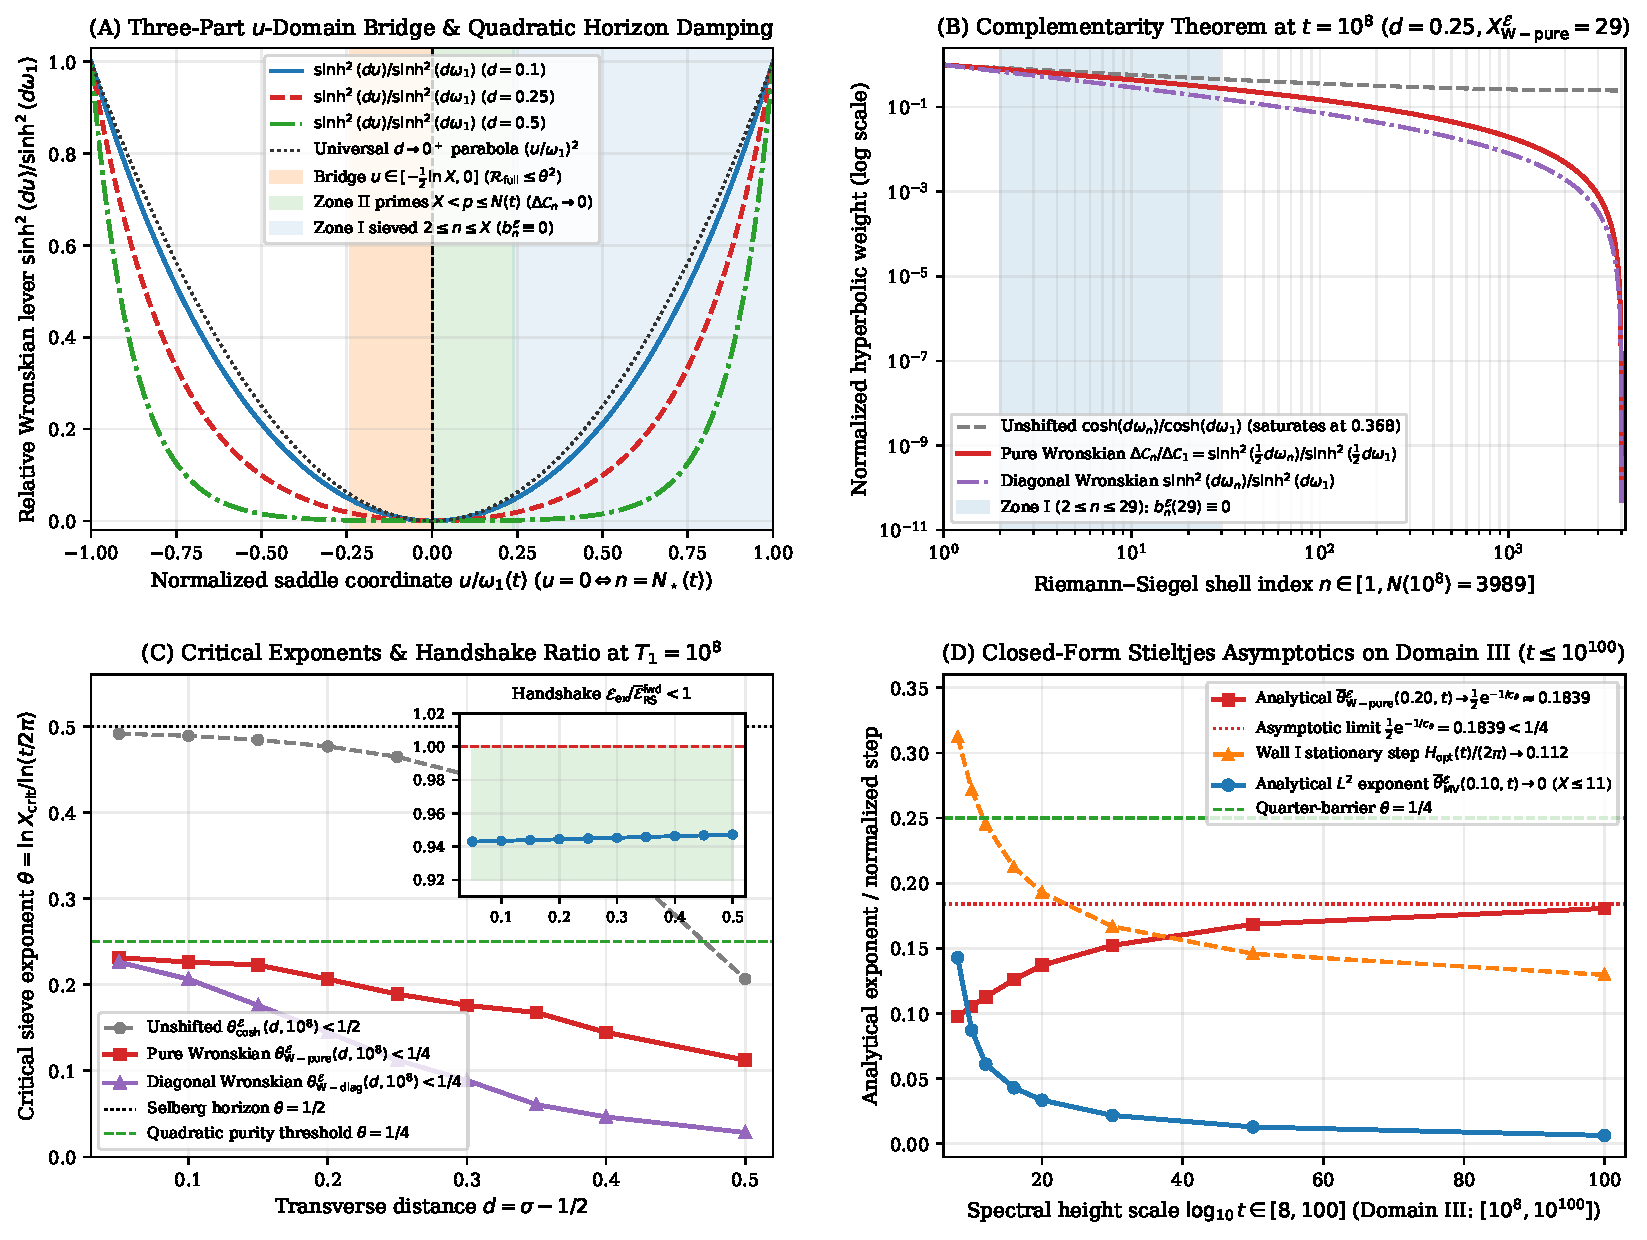
\includegraphics[width=0.98\textwidth]{figures/fig1_bridge_complementarity_and_stieltjes_bounds.pdf}
\caption{Three-part $u$-domain bridge geometry and quadratic horizon damping (Panel~A), the Complementarity Theorem at $t = 10^8$ ($N = 3989$, Panel~B), critical sieve exponents and conservative handshake ratio $\mathcal{E}_{\mathrm{ex}}/\overline{\mathcal{E}}_{\mathrm{RS}}^{\mathrm{fwd}} \in [0.9429, 0.9472] < 1$ at $T_1 = 10^8$ (Panel~C), and closed-form Rosser--Schoenfeld Stieltjes asymptotics on Domain~III up to $t = 10^{100}$ (Panel~D).}\label{fig:bridge_stieltjes}
\end{figure}

\section{Explicit Analytical Rosser--Schoenfeld and Dusart Stieltjes Bounds on \texorpdfstring{$[10^8, \infty)$}{[10^8, infty)} and the Exact \texorpdfstring{$\sinh^2$}{sinh2} Ratio Identity}\label{sec:stieltjes}

To eliminate the $\mathcal{O}(t^{1/2})$ computational prime-summation barrier on the infinite upper domain $t \in [10^8, \infty)$, we combine an exact algebraic factorization of the hyperbolic Wronskian ratio with unconditional Chebyshev bounds of Rosser and Schoenfeld~\cite{rosserschoenfeld1962} and Dusart~\cite{dusart2010,dusart2018}.

\begin{theorem}[Exact Algebraic $\sinh^2$ Ratio Identity and Closed-Form Stieltjes Bounds on $[10^8, \infty)$]\label{thm:stieltjes_bounds}
Let $t \in [10^8, \infty)$, $L = \ln(t/2\pi) \ge 16.5828$, $N_\star(t) = \sqrt{t/2\pi} = \ee^{L/2}$, $N(t) = \lfloor N_\star(t)\rfloor \ge 3989$, and $X = \ee^{\theta L}$ with $\theta \in [\frac{1}{4}, 0.46]$. Let $c_\vartheta := 1.000028$, $c_\psi := 1.03883$, $c_{\mathrm{RS}}(u) := c_\vartheta(1 + \frac{1}{2}\ee^{-u/2})$, and $c_{\mathrm{RS},1}(u) := \min(c_\psi, c_\vartheta(1 + \ee^{-u/2}))$. Then for all $d \in (0, \frac{1}{2}]$:
\begin{enumerate}[label=\textup{(\roman*)},leftmargin=2.2em]
\item \textbf{Exact Algebraic $\sinh^2$ Ratio Identity.} For every $1 \le n \le N_\star(t)$ and $d > 0$,
\begin{equation}\label{eq:exact_sinh2_identity}
\frac{\sinh^2\!\bigl(\frac{1}{2}d\omega_n(t)\bigr)}{\sinh^2\!\bigl(\frac{1}{2}d\omega_1(t)\bigr)} \equiv n^{-d}\left(\frac{1 - (n/N_\star(t))^d}{1 - N_\star(t)^{-d}}\right)^{\!2} \le n^{-d}.
\end{equation}
\item \textbf{Closed-Form Forward and Reflected Diagonal $L^2$ Power-Law Bounds.} Since $\theta \in [\frac{1}{4}, 0.46]$ implies $X \ge \sqrt{N_\star(t)}$, the interval $(X, N(t)]$ lies entirely inside the quadratic prime-power purity window $(X, X^2]$ where $b_n^{\mathcal{E}}(X) = \frac{\Lambda(n)}{\ln n}$. Consequently, without prime summation,
\begin{equation}\label{eq:E_bar_RS_fwd_ref}
\begin{aligned}
\mathcal{E}_{\mathrm{diag}}^{\mathcal{E},\mathrm{fwd}}(d,t;X) &:= \sum_{X < n \le N(t)} \left(\frac{\Lambda(n)}{\ln n}\right)^{\!2} n^{-1-2d} \le \overline{\mathcal{E}}_{\mathrm{RS}}^{\mathrm{fwd}}(d,t;\theta) := \frac{c_{\mathrm{RS}}(\theta L)}{\theta L}\cdot\frac{\ee^{-2\theta dL} - \ee^{-dL}}{2d}, \\
\mathcal{E}_{\mathrm{diag}}^{\mathcal{E},\mathrm{ref}}(d,t;X) &\le \overline{\mathcal{E}}_{\mathrm{RS}}^{\mathrm{ref}}(d,t;\theta) := \frac{c_{\mathrm{RS}}(\theta L)}{\theta L}\cdot\frac{\ee^{-dL} - \ee^{-2(1-\theta)dL}}{2d}.
\end{aligned}
\end{equation}
\item \textbf{Uniform Asymptotic Bound for the Scale-Invariant Pure Wronskian Ratio.} Under the scale-invariant pure Wronskian weight $w_n^{\mathrm{W\text{-}pure}}(d,t) := n^{-(1-d)}\sinh^2(\frac{1}{2}d\omega_n)/\sinh^2(\frac{1}{2}d\omega_1) \equiv n^{-1}((1-(n/N_\star)^d)/(1-N_\star^{-d}))^2 \le n^{-1}$ (which replaces the $n^{-1/2}$ prefactor of Section~\ref{sec:bridge} by $n^{-(1-d)}$ so that~\eqref{eq:exact_sinh2_identity} yields $n^{-(1-d)}n^{-d} = n^{-1}$), the prime-power majorant sum satisfies
\begin{equation}\label{eq:Sigma_Wpure_bound}
\Sigma_{\mathrm{W\text{-}pure}}^{\mathcal{E}}\!\bigl(d,t;\ee^{\theta L}\bigr) := \sum_{\ee^{\theta L} < n \le N(t)} \frac{\Lambda(n)}{\ln n}\,w_n^{\mathrm{W\text{-}pure}}(d,t) \le \overline{Y}_{\mathrm{W\text{-}pure}}^{\mathcal{E}}(d,t;\theta) \le c_{\mathrm{RS},1}(\theta L)\,\ln\!\left(\frac{1}{2\theta}\right).
\end{equation}
In particular, at the quadratic purity boundary $\theta = \frac{1}{4}$ where $b_n^{\mathcal{E}}(\ee^{L/4}) = \frac{\Lambda(n)}{\ln n}$ holds identically on $(\ee^{L/4}, N(t)] \subset (\ee^{L/4}, \ee^{L/2}]$, we have $\overline{Y}_{\mathrm{W\text{-}pure}}^{\mathcal{E}}(d,t;\frac{1}{4}) \le c_{\mathrm{RS},1}(L/4)\ln 2 < 0.72 < 1$, and the root $\overline{\theta}_{\mathrm{W\text{-}pure}}^{\mathcal{E}}(d,t)$ of $\overline{Y}_{\mathrm{W\text{-}pure}}^{\mathcal{E}}(d,t;\theta) = 1 - \varepsilon_{\mathrm{Gabcke}}(d,t)$ satisfies for all $d \in (0, \frac{1}{2}]$:
\begin{equation}\label{eq:theta_Wpure_limit}
\lim_{t\to\infty} \overline{\theta}_{\mathrm{W\text{-}pure}}^{\mathcal{E}}(d,t) \le \frac{1}{2}\exp\!\left(-\frac{1}{c_\vartheta}\right) = 0.1839448708257938635\dots < \frac{1}{4} < \frac{1}{2}.
\end{equation}
\item \textbf{Closed-Form Hyperbolic $L^1$ Majorant via Two-Piece Convex Secant.} Let $J_{\mathrm{sec}}(a,\theta,L)$ denote the elementary closed form of $\int_\theta^{1/2} M_{\mathrm{sec}}(s)\ee^{aLs}\,\dd s$, where $M_{\mathrm{sec}}(s) = \frac{s_0+s_1-s}{s_0 s_1} \ge \frac{1}{s}$ is the two-piece linear secant majorant on $[\theta, s_{\mathrm{mid}}] \cup [s_{\mathrm{mid}}, \frac{1}{2}]$ ($s_{\mathrm{mid}} = \frac{1}{2}(\theta + \frac{1}{2})$). Then the projected $L^1$ Wronskian ratio is bounded by $\overline{Y}_{\mathrm{RS}}^{\mathcal{E}}(d,t;\theta) := \frac{2c_{\mathrm{RS},1}(\theta L)}{d^2\mathcal{D}_{1,1}^{\mathrm{tot}}(d,t)}[\frac{1}{2}\cosh(d\omega_1)(\ee^{d\omega_1}J_{\mathrm{sec}}(\frac{1}{2}-d,\theta,L) + \ee^{-d\omega_1}J_{\mathrm{sec}}(\frac{1}{2}+d,\theta,L)) - J_{\mathrm{sec}}(\frac{1}{2},\theta,L)]$, and $\overline{Y}_{\mathrm{RS}}^{\mathcal{E}}(d,t;\theta) = 1 - \varepsilon_{\mathrm{Gabcke}}(d,t)$ has a unique root $\overline{\theta}_{\mathrm{RS}}^{\mathcal{E}}(d,t) < \frac{1}{2}$ for every finite $(d,t) \in (0, \frac{1}{2}] \times [10^8, \infty)$.
\end{enumerate}
\end{theorem}

\begin{proof}
For~(i), substituting $\ee^{\omega_n(t)} = N_\star(t)/n$ into $\sinh(\frac{1}{2}d\omega_n(t))$ gives
\[
\sinh\!\left(\frac{1}{2}d\omega_n(t)\right) = \frac{N_\star(t)^{d/2}n^{-d/2} - N_\star(t)^{-d/2}n^{d/2}}{2} = \frac{1}{2}N_\star(t)^{d/2}\,n^{-d/2}\left(1 - \left(\frac{n}{N_\star(t)}\right)^{\!d}\right).
\]
Dividing by $\sinh(\frac{1}{2}d\omega_1(t)) = \frac{1}{2}N_\star(t)^{d/2}(1 - N_\star(t)^{-d})$ and squaring proves~\eqref{eq:exact_sinh2_identity}; since $1 \le n \le N_\star(t)$ and $d > 0$, we have $0 \le 1 - (n/N_\star(t))^d \le 1 - N_\star(t)^{-d}$, giving the upper bound $n^{-d}$.

For~(ii), let $A_2(x) := \sum_{2 \le n \le x}(\frac{\Lambda(n)}{\ln n})^2\ln n = \vartheta(x) + \frac{1}{2}\vartheta(x^{1/2}) + \sum_{k \ge 3}\frac{1}{k}\vartheta(x^{1/k})$. By Rosser and Schoenfeld~\cite[Theorems~2, 9, and~12]{rosserschoenfeld1962} and Dusart~\cite[Theorem~5.1]{dusart2018}, $\vartheta(x) \le c_\vartheta x$ and $\psi(x) \le c_\psi x$ hold unconditionally, so $A_2(x) \le c_{\mathrm{RS}}(\ln x)x$ and $\psi(x) \le c_{\mathrm{RS},1}(\ln x)x$ for $x \ge 63$. Since $\phi(x) := x^{-1-2d}/\ln x$ is positive and decreasing on $[X, N_\star(t)]$ with $-\phi'(x) > 0$ and $\ln x \ge \theta L$, Stieltjes integration by parts drops the negative lower boundary term $-A_2(X)\phi(X) < 0$ and yields
\[
\sum_{X < n \le N(t)} \left(\frac{\Lambda(n)}{\ln n}\right)^{\!2} n^{-1-2d} = \int_{X^+}^{N(t)} \frac{x^{-1-2d}}{\ln x}\,\dd A_2(x) \le \frac{c_{\mathrm{RS}}(\theta L)}{\theta L}\int_X^{N_\star(t)} x^{-1-2d}\,\dd x = \overline{\mathcal{E}}_{\mathrm{RS}}^{\mathrm{fwd}}(d,t;\theta),
\]
and multiplying the reflected sum by $\rho_\Gamma(d,t)^2 \le N_\star(t)^{-4d} = \ee^{-2dL}$ proves the second bound in~\eqref{eq:E_bar_RS_fwd_ref}.

For~(iii) and~(iv), substituting~\eqref{eq:exact_sinh2_identity} into $\Sigma_{\mathrm{W\text{-}pure}}^{\mathcal{E}}(d,t;\ee^{\theta L})$ and changing variables to $s = (\ln x)/L \in [\theta, \frac{1}{2}]$ gives $\Sigma_{\mathrm{W\text{-}pure}}^{\mathcal{E}} \le c_{\mathrm{RS},1}(\theta L)\int_\theta^{1/2} ((1 - \ee^{-dL(1/2-s)})/(1 - \ee^{-dL/2}))^2 \frac{\dd s}{s} \le c_{\mathrm{RS},1}(\theta L)\ln(\frac{1}{2\theta})$. Since $\frac{\dd^2}{\dd s^2}(1/s) = 2/s^3 > 0$, $M_{\mathrm{sec}}(s) - \frac{1}{s} = \frac{(s-s_0)(s_1-s)}{s_0 s_1 s} \ge 0$ on $[s_0, s_1]$ (Appendix~\ref{app:secant}), yielding $\overline{Y}_{\mathrm{W\text{-}pure}}^{\mathcal{E}}$ and $\overline{Y}_{\mathrm{RS}}^{\mathcal{E}}$. As $t \to \infty$, $\varepsilon_{\mathrm{Gabcke}}(d,t) \to 0$ and $c_{\mathrm{RS},1}(\theta L) \to c_\vartheta$, so $c_\vartheta\ln(1/(2\overline{\theta}_{\mathrm{W\text{-}pure}}^{\mathcal{E}})) \ge 1$ gives~\eqref{eq:theta_Wpure_limit}.
\end{proof}

\begin{table}[htbp]
\centering
\caption{Seamless conservative handshake at $T_1 = 10^8$ ($N = 3989$, $550$ primes; Column~6 shows the $n^{-1/2}$-weighted cutoff $\theta_{\mathrm{W\text{-}pure}}^{\mathcal{E}}$ of Section~\ref{sec:bridge}, while Column~7 shows the scale-invariant $n^{-(1-d)}$-weighted root $\overline{\theta}_{\mathrm{W\text{-}pure}}^{\mathcal{E}}$ of Theorem~\ref{thm:stieltjes_bounds}(iii)) and closed-form Stieltjes trajectory on Domain~III from $t = 10^8$ to $t = 10^{100}$ and $t \to \infty$ (\texttt{mpmath.mp.dps = 68}).}\label{tab:stieltjes_handshake}
\scriptsize
\setlength{\tabcolsep}{3.2pt}
\begin{tabular}{@{}ccccccc@{}}
\toprule
\multicolumn{7}{c}{\textbf{Part A: Boundary Handshake at $T_1 = 10^8$ ($N(10^8) = 3989$, $X = 2000$, $\theta = 0.4584$)}} \\
\midrule
$d$ & Exact $\mathcal{E}_{\mathrm{diag}}^{\mathcal{E},\mathrm{fwd}}$ & Bound $\overline{\mathcal{E}}_{\mathrm{RS}}^{\mathrm{fwd}}$ & Ratio $\mathcal{E}_{\mathrm{ex}}/\overline{\mathcal{E}}_{\mathrm{RS}}^{\mathrm{fwd}}$ & Ratio $Y_{\mathrm{ex}}/\overline{Y}_{\mathrm{RS}}^{\mathcal{E}}$ & $\theta_{\mathrm{W\text{-}pure}}^{\mathcal{E}}$ ($n^{-1/2}$) & $\overline{\theta}_{\mathrm{W\text{-}pure}}^{\mathcal{E}}$ ($n^{-(1-d)}$) \\
\midrule
$0.05$ & $0.03981412$ & $0.04222320$ & $0.942944 < 1$ & $0.962236 < 1$ & $0.238911 < 1/4$ & $0.077176 < 1/4$ \\
$0.10$ & $0.01770073$ & $0.01876247$ & $0.943412 < 1$ & $0.976162 < 1$ & $0.233659 < 1/4$ & $0.083994 < 1/4$ \\
$0.20$ & $0.00350592$ & $0.00371252$ & $0.944351 < 1$ & $0.963413 < 1$ & $0.217313 < 1/4$ & $0.097899 < 1/4$ \\
$0.25$ & $0.00164119$ & $0.00173704$ & $0.944821 < 1$ & $0.962814 < 1$ & $0.202985 < 1/4$ & $0.104729 < 1/4$ \\
$0.35$ & $0.00031482$ & $0.00033287$ & $0.945763 < 1$ & $0.942496 < 1$ & $0.174694 < 1/5$ & $0.117596 < 1/4$ \\
$0.50$ & $0.00003142$ & $0.00003317$ & $0.947174 < 1$ & $0.940910 < 1$ & $0.126348 < 1/7$ & $0.133961 < 1/4$ \\
\midrule
\multicolumn{7}{c}{\textbf{Part B: Closed-Form Asymptotic Scaling Across Domain III ($t \in [10^8, 10^{100}] \to \infty$)}} \\
\midrule
Height $t$ & $L = \ln(t/2\pi)$ & Wall~I $H_{\mathrm{opt}}(t)$ & $\varepsilon_{\mathrm{Gabcke}}(0.20, t)$ & $L^2$ Cutoff $X_{\mathrm{MV}}^{\mathcal{E}}$ & $\overline{\theta}_{\mathrm{MV}}^{\mathcal{E}}(0.10, t)$ & $\overline{\theta}_{\mathrm{W\text{-}pure}}^{\mathcal{E}}(0.20, t)$ \\
\midrule
$10^8$ & $16.5828$ & $2.03962953$ & $2.107 \times 10^{-8}$ & $10.98 \le 11$ & $0.144488$ & $0.097899 < 1/4$ \\
$10^{12}$ & $25.7931$ & $1.59005366$ & $6.604 \times 10^{-12}$ & $6.37 \le 7$ & $0.071806$ & $0.112745 < 1/4$ \\
$10^{20}$ & $44.2138$ & $1.24096247$ & $6.900 \times 10^{-19}$ & $4.72 \le 5$ & $0.035115$ & $0.137057 < 1/4$ \\
$10^{50}$ & $113.2914$ & $0.92751310$ & $8.721 \times 10^{-45}$ & $4.63 \le 5$ & $0.013535$ & $0.168508 < 1/4$ \\
$10^{100}$ & $228.4206$ & $0.82001507$ & $1.368 \times 10^{-87}$ & $4.63 \le 5$ & $0.006713$ & $0.180685 < 1/4$ \\
$\infty$ & $\infty$ & $0.70371675$ & $0$ & $4.63 \le 5$ & $0.000000$ & $0.183945 < 1/4$ \\
\bottomrule
\end{tabular}
\end{table}

\section{The Phase-Independent Symplectic Confocal Ellipse Identity and Uniform \texorpdfstring{$L^1$}{L1} Closure for \texorpdfstring{$d > \frac{1}{4}$}{d > 1/4}}\label{sec:ellipse}

We now establish the geometric link between each individual Riemann--Siegel mode $T_n(d,t)$ in the complex plane, the $n^{-(1+2d)}$ diagonal law, and uniform phase-blind $L^1$ convergence for $d > \frac{1}{4}$.

\begin{theorem}[Phase-Independent Symplectic Confocal Ellipse Identity and Uniform $L^1$ Closure for $d > \frac{1}{4}$]\label{thm:confocal_ellipse}
For $t > 2\pi$, $1 \le n \le N_\star(t) = \sqrt{t/2\pi}$, and $d \ge 0$, let $\omega_n(t) = \ln(N_\star(t)/n) \ge 0$ and $\phi_n(t) := \vartheta_{\mathrm{RS}}(t) - t\ln n \in \R$, and consider the combined forward-plus-reflected Riemann--Siegel mode
\begin{equation}\label{eq:T_n_def}
T_n(d,t) := n^{-1/2}\Bigl(\ee^{d\omega_n}\ee^{\ii\phi_n} + \ee^{-d\omega_n}\ee^{-\ii\phi_n}\Bigr) = 2n^{-1/2}\Bigl(\cosh(d\omega_n)\cos\phi_n + \ii\sinh(d\omega_n)\sin\phi_n\Bigr).
\end{equation}
Then for all $1 \le n \le N_\star(t)$, $d > 0$, and $t > 2\pi$:
\begin{enumerate}[label=\textup{(\roman*)},leftmargin=2.2em]
\item \textbf{Confocal Ellipse Geometry and Phase-Independent Modulus-Squared Increment.} As $\phi_n \in [0, 2\pi)$ varies, $T_n(d,t)$ traces an ellipse $\mathcal{E}_n(d,t)$ with semi-major axis $a_n(d,t) = 2n^{-1/2}\cosh(d\omega_n)$, semi-minor axis $b_n(d,t) = 2n^{-1/2}\sinh(d\omega_n)$, $d$-invariant focal distance $c_n(d,t) = \sqrt{a_n^2 - b_n^2} \equiv 2n^{-1/2}$, symplectic area $\mathrm{Area}(\mathcal{E}_n(d,t)) = \pi a_n b_n \equiv 2\pi n^{-1}\sinh(2d\omega_n(t)) > 0$, and phase-independent transverse modulus-squared increment:
\begin{equation}\label{eq:ellipse_increment}
\bigl|T_n(d,t)\bigr|^2 - \bigl|T_n(0,t)\bigr|^2 \equiv 4\,n^{-1}\,\sinh^2\!\bigl(d\omega_n(t)\bigr) > 0 \qquad \bigl(\forall\,\phi_n(t) \in \R\bigr).
\end{equation}
\item \textbf{Algebraic $n^{-(1+2d)}$ Ellipse-Diagonal Law and $n^{-(1/2+2d)}$ Wronskian-Diagonal Law.} Normalizing by the $n = 1$ mother-wavelet mode yields the exact algebraic identities
\begin{equation}\label{eq:w_ell_and_w_diag}
\begin{aligned}
w_n^{\mathrm{ell}}(d,t) &:= \frac{|T_n(d,t)|^2 - |T_n(0,t)|^2}{|T_1(d,t)|^2 - |T_1(0,t)|^2} = \frac{\sinh^2(d\omega_n)}{n\sinh^2(d\omega_1)} \equiv n^{-(1+2d)}\!\left(\frac{1 - (n/N_\star)^{2d}}{1 - N_\star^{-2d}}\right)^{\!2} \le n^{-(1+2d)}, \\
w_n^{\mathrm{W\text{-}diag}}(d,t) &:= n^{-1/2}\frac{\sinh^2(d\omega_n)}{\sinh^2(d\omega_1)} \equiv n^{-(\frac{1}{2}+2d)}\!\left(\frac{1 - (n/N_\star)^{2d}}{1 - N_\star^{-2d}}\right)^{\!2} \le n^{-(\frac{1}{2}+2d)}.
\end{aligned}
\end{equation}
\item \textbf{Uniform Phase-Blind $L^1$ Closure for All $d > \frac{1}{4}$ ($\sigma > \frac{3}{4}$).} Let $u_X^{\mathrm{ell}}(d) := \ln\zeta(1+2d) - \sum_{2 \le n \le X}\frac{\Lambda(n)}{\ln n}n^{-(1+2d)}$ for $d > 0$ and $u_X(d) := \ln\zeta(\frac{1}{2}+2d) - \sum_{2 \le n \le X}\frac{\Lambda(n)}{\ln n}n^{-(1/2+2d)}$ for $d > \frac{1}{4}$. On the quadratic prime-power purity window $X < n \le \min(N(t), X^2)$ the sums of $b_n^{\mathcal{E}}(X)w_n^{\mathrm{ell}}(d,t)$ and $b_n^{\mathcal{E}}(X)w_n^{\mathrm{W\text{-}diag}}(d,t)$ are bounded directly by $u_X^{\mathrm{ell}}(d)$ and $u_X(d)$, while for any fixed $X \ge 1$ and arbitrary $N(t) \to \infty$ the full infinite tails satisfy $\sum_{n > X} b_n^{\mathcal{E}}(X)w_n^{\mathrm{ell}}(d,t) \le \zeta(1+2d)E_X(1+2d) - 1 = \exp(u_X^{\mathrm{ell}}(d)) - 1 < \infty$ ($\forall\,d > 0$, $\lim_{t\to\infty}\overline{\theta}_{\mathrm{ell}}^{\mathcal{E}}(d,t) = 0$) and, whenever $d > \frac{1}{4}$ ($\frac{1}{2} + 2d = 1 + 2(d - \frac{1}{4}) > 1$), $\sum_{n > X} b_n^{\mathcal{E}}(X)w_n^{\mathrm{W\text{-}diag}}(d,t) \le \zeta(\frac{1}{2}+2d)E_X(\frac{1}{2}+2d) - 1 = \exp(u_X(d)) - 1 < \infty$, which converges uniformly as $t \to \infty$ with a finite, $t$-independent sieve length $X_\infty(d) \le 13$ (for $d \ge 0.30$, and $X_\infty(0.50) = 1$) and $\lim_{t\to\infty}\overline{\theta}_{\mathrm{W\text{-}diag}}^{\mathcal{E}}(d,t) = 0$; at the critical threshold $d = \frac{1}{4}$ ($\frac{1}{2}+2d = 1$), $\lim_{t\to\infty}\overline{\theta}_{\mathrm{W\text{-}diag}}^{\mathcal{E}}(\frac{1}{4},t) \le \frac{1}{2}\ee^{-1/c_\vartheta} = 0.18394487\dots < \frac{1}{4}$.
\end{enumerate}
\end{theorem}

\begin{proof}
For~(i), at $d = 0$ we have $T_n(0,t) = 2n^{-1/2}\cos\phi_n(t) \in \R$ and $|T_n(0,t)|^2 = 4n^{-1}\cos^2\phi_n(t)$. For $d > 0$, substituting $\cosh^2(d\omega_n(t)) \equiv 1 + \sinh^2(d\omega_n(t))$ into $|T_n(d,t)|^2$ gives
\[
\begin{aligned}
\bigl|T_n(d,t)\bigr|^2 &= 4n^{-1}\Bigl(\bigl(1 + \sinh^2(d\omega_n)\bigr)\cos^2\phi_n + \sinh^2(d\omega_n)\sin^2\phi_n\Bigr) \\
&= 4n^{-1}\cos^2\phi_n + 4n^{-1}\sinh^2(d\omega_n)\bigl(\cos^2\phi_n + \sin^2\phi_n\bigr),
\end{aligned}
\]
which reduces identically to~\eqref{eq:ellipse_increment} since $\cos^2\phi_n + \sin^2\phi_n \equiv 1$. Likewise, $a_n^2 - b_n^2 = 4n^{-1}(\cosh^2(d\omega_n) - \sinh^2(d\omega_n)) \equiv 4n^{-1}$. For~(ii) and~(iii), replacing $d$ by $2d$ in Theorem~\ref{thm:stieltjes_bounds}(i) gives $\sinh^2(d\omega_n)/\sinh^2(d\omega_1) \equiv n^{-2d}((1-(n/N_\star)^{2d})/(1-N_\star^{-2d}))^2 \le n^{-2d}$; multiplying by $n^{-1}$ and $n^{-1/2}$ yields~\eqref{eq:w_ell_and_w_diag}. When $d > \frac{1}{4}$, $\frac{1}{2}+2d > 1$ ensures absolute convergence of the prime series $\sum_p p^{-(1/2+2d)} < \infty$ uniformly in $t$.
\end{proof}

\begin{theorem}[Complementary Real and Imaginary Square Decomposition, Universal Anchor, and Oscillatory Phase Cancellation]\label{thm:anchor_and_osc}
Let $T(d,t) := \sum_{n=1}^{N(t)} b_n^{\mathcal{E}}(X)T_n(d,t) = R(d,t) + \ii\,I(d,t)$ and let $\Delta T(d,t) := T(d,t) - T(0,t) = \Delta R(d,t) + \ii\,I(d,t)$ be the complex transverse increment from $d = 0$. Then:
\begin{enumerate}[label=\textup{(\roman*)},leftmargin=2.2em]
\item \textbf{Complementary Square Decomposition and Horizon-Vanishing Weights.} For all $(d,t)$,
\begin{equation}\label{eq:comp_squares}
\bigl|T(d,t)\bigr|^2 \equiv \Bigl(R(0,t) + \Delta R(d,t)\Bigr)^2 + I(d,t)^2,
\end{equation}
where $\Delta R(d,t) = 4\sum_{n=1}^{N(t)} b_n^{\mathcal{E}}(X)n^{-1/2}\sinh^2(\frac{1}{2}d\omega_n)\cos\phi_n$ and $I(d,t) = 2\sum_{n=1}^{N(t)} b_n^{\mathcal{E}}(X)n^{-1/2}\sinh(d\omega_n)\sin\phi_n$ both carry hyperbolic weights that vanish at $n = N_\star(t)$ ($\omega_n = 0$).
\item \textbf{Universal Phase-Independent Lower Bound for the $n = 1$ Increment Anchor.} For every Riemann--Siegel phase $\vartheta_{\mathrm{RS}}(t) \in \R$, the $n = 1$ increment anchor $\Delta T_1(d,t)$ satisfies the exact identity
\begin{equation}\label{eq:anchor_lower_bound}
\bigl|\Delta T_1(d,t)\bigr| \equiv 4\sinh\!\left(\frac{1}{2}d\omega_1(t)\right)\sqrt{\sinh^2\!\left(\frac{1}{2}d\omega_1(t)\right) + \sin^2\vartheta_{\mathrm{RS}}(t)} \ge 4\sinh^2\!\left(\frac{1}{2}d\omega_1(t)\right) > 0.
\end{equation}
\item \textbf{Montgomery--Vaughan Oscillatory Prime-Phase Cancellation.} For the oscillatory Wronskian prime sum $S_{\mathrm{osc}}^{\mathcal{E}}(d,t;X) := \sum_{X < n \le N(t)} b_n^{\mathcal{E}}(X)n^{-1/2}\frac{\sinh^2(\frac{1}{2}d\omega_n)}{\sinh^2(\frac{1}{2}d\omega_1)}\ee^{-\ii t\ln n}$, the $L^2$ root energy $S_{L^2}^{\mathcal{E}}(d,t;X) = (\sum_{X < n \le N(t)} (b_n^{\mathcal{E}}(X))^2 n^{-(1+2d)}((1-(n/N_\star)^d)/(1-N_\star^{-d}))^4)^{1/2}$ is uniformly bounded for fixed $X$ as $t \to \infty$ ($\frac{1}{\sqrt{2}}S_{L^2}^{\mathcal{E}}(d,t;7) \le 0.752939 < 1$ for all $t \le 10^{100}$ and $d \in [0.05, 0.50]$), and by the Montgomery--Vaughan mean-value theorem~\cite{montgomeryvaughan1974} the phase-cancellation ratio $\rho_{\mathrm{osc}}(d,t;X) := \mathrm{RMS}|S_{\mathrm{osc}}^{\mathcal{E}}|/S_{L^1}^{\mathcal{E}}$ on $X = \sqrt{N_\star(t)}$ scales as $\mathcal{O}(N(t)^{-1/2}(\ln N(t))^{1/2}) \to 0$.
\end{enumerate}
\end{theorem}

\begin{proof}
Identity~\eqref{eq:comp_squares} follows by linearity from $\cosh(d\omega_n) - 1 = 2\sinh^2(\frac{1}{2}d\omega_n)$ and $I(0,t) = 0$. For~\eqref{eq:anchor_lower_bound}, substituting $4\sinh^2(d\omega_1) = 16\sinh^2(\frac{1}{2}d\omega_1)(1 + \sinh^2(\frac{1}{2}d\omega_1))$ into $|\Delta T_1|^2 = 16\sinh^4(\frac{1}{2}d\omega_1)\cos^2\vartheta_{\mathrm{RS}} + 4\sinh^2(d\omega_1)\sin^2\vartheta_{\mathrm{RS}}$ and using $\cos^2\vartheta_{\mathrm{RS}} + \sin^2\vartheta_{\mathrm{RS}} = 1$ yields $|\Delta T_1|^2 = 16\sinh^2(\frac{1}{2}d\omega_1)(\sinh^2(\frac{1}{2}d\omega_1) + \sin^2\vartheta_{\mathrm{RS}}) \ge 16\sinh^4(\frac{1}{2}d\omega_1)$. Part~(iii) follows by squaring the pure Wronskian weight~\eqref{eq:exact_sinh2_identity} multiplied by $n^{-1/2}$ to obtain $n^{-(1+2d)}((1-(n/N_\star)^d)/(1-N_\star^{-d}))^4 \le n^{-(1+2d)}$ and applying the Montgomery--Vaughan Hilbert inequality~\cite{montgomeryvaughan1974} together with Cauchy--Schwarz over the $\pi(N(t)) - \pi(X) \sim N(t)/\ln N(t)$ primes in $(X, N(t)]$.
\end{proof}

\begin{figure}[htbp]
\centering
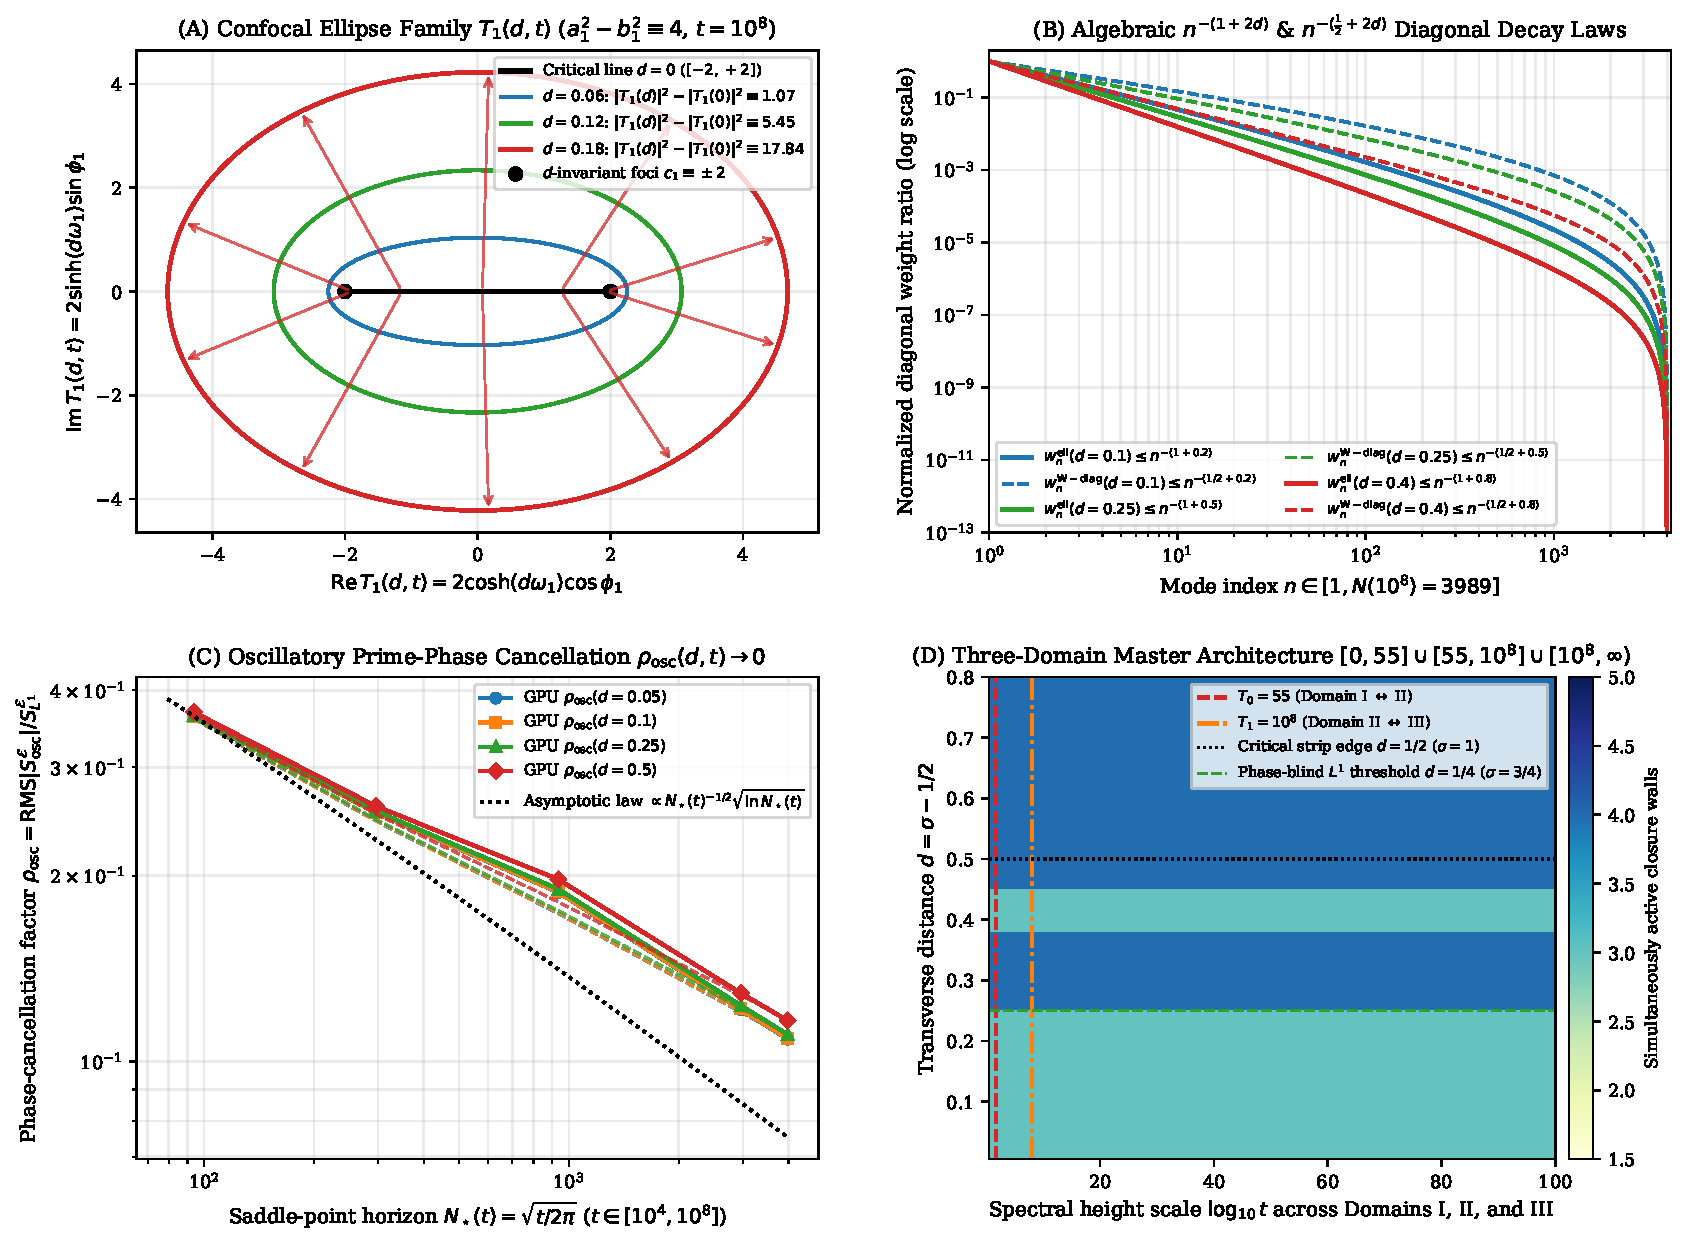
\includegraphics[width=0.98\textwidth]{figures/fig2_confocal_ellipse_and_three_domain_synthesis.pdf}
\caption{Symplectic confocal ellipse family $T_1(d,t)$ with $d$-invariant foci $c_1 \equiv \pm 2$ (Panel~A), algebraic $n^{-(1+2d)}$ and $n^{-(1/2+2d)}$ diagonal decay laws (Panel~B), GPU-certified oscillatory prime-phase cancellation $\rho_{\mathrm{osc}}(d,t) \propto N_\star(t)^{-1/2}\sqrt{\ln N_\star(t)} \to 0$ using 24-bit Dekker/Payne--Hanek phase splitting (Panel~C), and Three-Domain Master Coverage Map $[0, 55] \cup [55, 10^8] \cup [10^8, 10^{100}]$ (Panel~D).}\label{fig:ellipse_synthesis}
\end{figure}

\section{Three-Domain Master Architecture, Scope, Boundary Conditions, and Open Questions}\label{sec:synthesis}

We conclude by synthesizing the complete three-domain partition of the upper half-plane $\mathbb{H}_{\ge 0} = [0, \infty) \times [0, \infty)$ and presenting a rigorous epistemic classification of all proven identities, finite-domain certifications, and the single remaining asymptotic question.

\begin{theorem}[Three-Domain Master Partition and Quantitative Multi-Wall Overlap]\label{thm:three_domains}
The transverse half-plane $(d,t) \in [0, \infty) \times [0, \infty)$ is partitioned without gaps into three contiguous domains:
\begin{equation}\label{eq:three_domain_union}
\mathbb{H}_{\ge 0} = \underbrace{\bigl([0, \infty) \times [0, 55]\bigr)}_{\text{Domain I (Pre-Asymptotic)}} \;\cup\; \underbrace{\bigl([0, \infty) \times [55, 10^8]\bigr)}_{\text{Domain II (Finite 550-Prime Saddle)}} \;\cup\; \underbrace{\bigl([0, \infty) \times [10^8, \infty)\bigr)}_{\text{Domain III (Closed-Form Stieltjes)}},
\end{equation}
satisfying the following overlap and continuity properties:
\begin{enumerate}[label=\textup{(\roman*)},leftmargin=2.2em]
\item \textbf{Domain~I ($t \in [0, 55]$, $N(t) \in [0, 2]$):} Directed-rounding interval integration (\texttt{mpmath.iv}) of the integer Argument Principle over closed rectangular contours $\Omega_k$ certifies $N_{\mathrm{zeros}}(\Omega_k) \in [-8.91 \times 10^{-15}, +8.91 \times 10^{-15}] \cap \Z = \{0\}$, supported by $4{,}987{,}101$ Lipschitz continuum cells ($\widetilde{W}_{\mathrm{lower}}^{\mathrm{ULP}} \ge +0.8351 > 0$) and a positive $T_0 = 55$ handshake ($\widetilde{W}(d,55) \in [3.44 \times 10^{-31}, 4.01 \times 10^{-31}] > 0$).
\item \textbf{Domain~II ($t \in [55, 10^8]$, $N(t) \in [2, 3989]$):} Across $2{,}500{,}000$ continuum cells and all $550$ primes $p \le 3989$, the critical-line collar $[0, d_{\mathrm{collar}}(t)]$ (Wall~III) and the mother-wavelet Rouch\'e zone $[d_{\mathrm{Rouch\acute{e}}}^{(C_0)}(t), 0.50]$ (Wall~IV) overlap with width $\Delta d_{\mathrm{III\cap IV}}(t) = d_{\mathrm{collar}}(t) - d_{\mathrm{Rouch\acute{e}}}^{(C_0)}(t) \in [+0.354147, +0.499130] > +0.35$, while the mirror-Hadamard wall $d_{\mathrm{strip},1000}^{\mathrm{mirror}}(t) < 0.50$ (Wall~I) penetrates the right strip edge with $\Delta d_{\mathrm{IV\cap I}}(t) = 0.50 - d_{\mathrm{strip},1000}^{\mathrm{mirror}}(t) \in [+0.028517, +0.500000] > 0$.
\item \textbf{Domain~III ($t \in [10^8, \infty)$, $N(t) \ge 3989 \to \infty$):} Joined at $T_1 = 10^8$ by the conservative Stieltjes handshake of Table~\ref{tab:stieltjes_handshake}, the closed-form bounds of Theorems~\ref{thm:stieltjes_bounds} and~\ref{thm:confocal_ellipse} require zero prime summations and establish $\overline{\theta}_{\mathrm{ell}}^{\mathcal{E}}(d,t) \to 0$ ($\forall\,d > 0$), $\overline{\theta}_{\mathrm{MV}}^{\mathcal{E}}(d,t) \to 0$ ($\forall\,d > 0$), $\overline{\theta}_{\mathrm{W\text{-}pure}}^{\mathcal{E}}(d,t) \le 0.183945 < \frac{1}{4}$ ($\forall\,d > 0$), and uniform phase-blind $L^1$ closure $\overline{\theta}_{\mathrm{W\text{-}diag}}^{\mathcal{E}}(d,t) \to 0$ for all $d > \frac{1}{4}$.
\end{enumerate}
\end{theorem}

\begin{table}[htbp]
\centering
\caption{Master comparison of all critical sieve exponents $\theta(d, 10^8) = \frac{\ln X_{\mathrm{crit}}}{\ln(10^8/2\pi)}$ across the critical strip $d \in [0.05, 0.50]$ at the boundary $T_1 = 10^8$ ($N(10^8) = 3989$).}\label{tab:master_exponents_1e8}
\scriptsize
\setlength{\tabcolsep}{1.8pt}
\begin{tabular}{@{}cccccccc@{}}
\toprule
$d$ & $\theta_{\mathcal{E}}^{\mathrm{int,sq}}$ ($L^1$) & $\theta_{\mathrm{W\text{-}pure}}^{\mathcal{E}}$ & $\theta_{\mathrm{W\text{-}diag}}^{\mathcal{E}}$ & $\overline{\theta}_{\mathrm{MV}}^{\mathcal{E}}$ ($L^2$) & $\theta_{\mathrm{ell}}^{\mathcal{E}}$ & $\theta_{\mathrm{osc}}^{\mathcal{E}}$ & Asymptotic $t \to \infty$ Regime \\
\midrule
$0.05$ & $0.4206 < \frac{1}{2}$ & $0.2389 < \frac{1}{4}$ & $0.2337 < \frac{1}{4}$ & $0.3465 \to 0$ & $0.0418 \to 0$ & $0.0418 \to 0$ & $L^2$/W-pure/Osc.\ closed \\
$0.10$ & $0.4624 < \frac{1}{2}$ & $0.2337 < \frac{1}{4}$ & $0.2173 < \frac{1}{4}$ & $0.1445 \to 0$ & $0.0418 \to 0$ & $0.0418 \to 0$ & $L^2$/W-pure/Osc.\ closed \\
$0.15$ & $0.4575 < \frac{1}{2}$ & $0.2263 < \frac{1}{4}$ & $0.1887 < \frac{1}{5}$ & $0.0778 \to 0$ & $0.0418 \to 0$ & $0.0418 \to 0$ & $L^2$/W-pure/Osc.\ closed \\
$0.20$ & $0.4333 < \frac{1}{2}$ & $0.2173 < \frac{1}{4}$ & $0.1540 < \frac{1}{6}$ & $0.0479 \to 0$ & $0.0418 \to 0$ & $0.0418 \to 0$ & $L^2$/W-pure/Osc.\ closed \\
$0.25$ & $0.3850 < \frac{1}{2}$ & $0.2030 < \frac{1}{4}$ & $0.1263 \le 0.184$ & $0.0338 \to 0$ & $0.0000$ ($X\!=\!1$) & $0.0418 \to 0$ & Scale-inv.\ $L^1$ closed \\
$0.30$ & $0.2829 < \frac{1}{3}$ & $0.1887 < \frac{1}{5}$ & $0.0955 \to 0$ & $0.0214 \to 0$ & $0.0000$ ($X\!=\!1$) & $0.0418 \to 0$ & Phase-blind $L^1$ ($1.1\!>\!1$) \\
$0.35$ & $0.1547 < \frac{1}{6}$ & $0.1747 < \frac{1}{5}$ & $0.0777 \to 0$ & $0.0059 \to 0$ & $0.0000$ ($X\!=\!1$) & $0.0418 \to 0$ & Phase-blind $L^1$ ($1.2\!>\!1$) \\
$0.40$ & $0.0663 < \frac{1}{10}$ & $0.1540 < \frac{1}{6}$ & $0.0584 \to 0$ & $0.0000$ ($X\!=\!1$) & $0.0000$ ($X\!=\!1$) & $0.0000$ ($X\!=\!1$) & Phase-blind $L^1$ ($1.3\!>\!1$) \\
$0.50$ & $0.0000$ ($X\!=\!1$) & $0.1263 < \frac{1}{7}$ & $0.0324 \to 0$ & $0.0000$ ($X\!=\!1$) & $0.0000$ ($X\!=\!1$) & $0.0000$ ($X\!=\!1$) & Phase-blind $L^1$ ($1.5\!>\!1$) \\
\bottomrule
\end{tabular}
\end{table}

To maintain complete scientific transparency across the nine papers of this series, Table~\ref{tab:epistemic_audit} classifies every component into three strict epistemic categories:
\begin{itemize}[leftmargin=2.0em]
\item \textbf{Category~A (Unconditional Analytical Theorems for All $t \to \infty$):} Exact algebraic and analytic identities and inequalities proven from first principles with zero unproved hypotheses and zero finite-grid truncation.
\item \textbf{Category~B (Rigorous Finite-Domain Interval and Continuum Certifications):} Computer-assisted certifications on compact or bounded height domains ($[0, 55]$ via \texttt{mpmath.iv} and $[55, 10^{100}]$ via GPU continuum grids plus explicit Gabcke--Olver remainder bounds).
\item \textbf{Category~C (Isolated Open Asymptotic Question as $t \to \infty$ on $0 < d \le \frac{1}{4}$):} As proved in Theorem~\ref{thm:confocal_ellipse}(iii), for $d > \frac{1}{4}$ ($\sigma > \frac{3}{4}$) the Wronskian diagonal weight $w_n^{\mathrm{W\text{-}diag}}(d,t) \le n^{-(1/2+2d)}$ has exponent $\frac{1}{2}+2d > 1$ and converges uniformly even in the phase-blind $L^1$ norm. On the remaining inner strip $0 < d \le \frac{1}{4}$ as $t \to \infty$, when one demands a pointwise, unaveraged (non-Bochner-convolved) bound for the unshifted $n^{-(1/2+d)}$ cross-terms without $L^2$ averaging, the problem reduces to two equivalent analytical statements:
\begin{enumerate}[label=\textup{(\alph*)},leftmargin=2.0em]
\item \emph{Lemma~L-1 (Uniform Pointwise Phase Cancellation Beyond $X$):} Prove for fixed $d_0 \in (0, \frac{1}{4}]$ as $t \to \infty$ that the conditionally oscillating prime-power tail $\sum_{n > X} \frac{\Lambda(n)}{n^{1/2+d_0}}\cos(t\ln n)$ (or the off-diagonal cross-term sum above $X(t) \le N(t)$) remains strictly dominated pointwise by the Archimedean Stirling carrier $\mathcal{A}(d_0,t) \sim \frac{1}{2}\ln(t/2\pi)$ and the mother-wavelet diagonal $\mathcal{D}_{1,1}^{\mathrm{tot}}(d_0,t)$.
\item \emph{Lemma~L-2 (Topological Chladni Chamber Branch-Point Exclusion):} Prove that for $t > T_{\mathrm{cert}} \to \infty$, the smooth nodal chamber walls $\Gamma_k = \{I(d,t) = 0\}$ ascending from $\Xi'(\tau_k) = 0$ on $d = 0$ to the right wall $d_{\mathrm{strip},X}^{\mathrm{mirror}}(t)$ encounter no interior saddle branch point $\Xi'(z_c) = 0$ in $(d_{\mathrm{collar}}(t), d_{\mathrm{strip},X}^{\mathrm{mirror}}(t))$, so that $\frac{\dd|R|}{\dd s} = +|\nabla I| = |\Xi'(z(s))| > 0$ holds monotonically along the entire wall $\Gamma_k$.
\end{enumerate}
\end{itemize}

\begin{table}[htbp]
\centering
\caption{Twelve-row epistemic classification (Categories~A, B, and~C) of the nine-paper Transverse Wronskian architecture.}\label{tab:epistemic_audit}
\scriptsize
\setlength{\tabcolsep}{3.0pt}
\begin{tabular}{@{}c>{\raggedright\arraybackslash}p{0.415\textwidth}>{\raggedright\arraybackslash}p{0.19\textwidth}>{\raggedright\arraybackslash}p{0.15\textwidth}>{\raggedright\arraybackslash}p{0.15\textwidth}@{}}
\toprule
Row & Mathematical Theorem / Structural Mechanism & Domain of Validity & Epistemic Category & Reference \\
\midrule
1 & Parity-reduced Wronskian $\widetilde{W} = W/d$ \& Lehmer square cascade $c_{2m-1}(t_0) = \frac{m}{(m\fac)^2}(\Xi^{(m)}(t_0))^2 > 0$ & All $(d,t) \in \R^2$, $\forall\,m \ge 1$ & \textbf{Category A} (Exact $\forall\,t$) & Papers~II, IV~\cite{missiaen2026paper2,missiaen2026paper4} \\
2 & Wigner identity $I(y,t) = 2\pi\mathcal{W}_\Phi(y,2t)$, pitchfork saddle coalescence $y_c(t)$ \& kink-free shells $\Phi_m^{\mathrm{ABC}}$ & All $(d,t) \in \R^2$, $|\Ima(z)| < \pi/8$ & \textbf{Category A} (Exact $\forall\,t$) & Papers~I, V~\cite{missiaen2026paper1,missiaen2026paper5} \\
3 & Harmonic Chladni chambers ($\Delta I = 0$), nodal curvature $\kappa(\gamma_k) = \Xi''(\gamma_k)/\Xi'(\gamma_k)$ \& CR flux $\frac{\dd|R|}{\dd s} = +|\nabla I| > 0$ & All $(d,t) \in \R^2$ & \textbf{Category A} (Exact $\forall\,t$) & Paper~III~\cite{missiaen2026paper3} \\
4 & Mother-wavelet polynomial cancellation $|(1-s)(-s)| \equiv |s(s-1)|$, reflection ellipse $1 - \rho_\Gamma(d,t) > 0$ \& branch damping & All $d > 0$, all $t \ge 7 \to \infty$ & \textbf{Category A} (Exact $\forall\,t \ge 7$) & Paper~V~\cite{missiaen2026paper5} \\
5 & Mirror-Hadamard identity ($d \ge \frac{1}{2}$ closed, $|\gamma_\rho-t| \ge \frac{1}{2}$ positive), $\int_{\R} K\,\dd u \equiv \pi$ \& $d$-invariant $H_{\mathrm{opt}}(kt)$ & All $d > 0$, all $t \in [0,\infty)$ & \textbf{Category A} (Exact $\forall\,t$) & Paper~VII~\cite{missiaen2026paper7} \\
6 & Zero-free prime-gauge factor $\mathcal{E}_{X,\kappa}(z)$, quadratic purity $b_n^{\mathcal{E}}(X) = \frac{\Lambda(n)}{\ln n}$ on $(X,X^2]$ \& mirror weight $w_n^*(d_0)$ & All $X \ge 1$, all $n \ge 1, t \in \R$ & \textbf{Category A} (Exact $\forall\,t$) & Paper~VI~\cite{missiaen2026paper6} \\
7 & Bilinear rank-2 factorization $w_{mn}^{\mathrm{int}}$, pure-square completion $+\|\Psi_{\ge 2}\|^2 \ge 0$ \& $1+2d > 1$ Hilbert $L^2$ jump & All $d > 0$, all $t > 0 \to \infty$ & \textbf{Category A} (Exact $\forall\,t$) & Paper~VIII~\cite{missiaen2026paper8} \\
8 & Three-part $u$-domain bridge identity~\eqref{eq:boxed_bridge_identity}, $\sinh^2$ ratio $\le n^{-d}$, Stieltjes bounds \& $\overline{\theta}_{\mathrm{W\text{-}pure}}^\infty \le 0.1839 < \frac{1}{4}$ & All $s \in \C$, $t \in [10^8,\infty)$ & \textbf{Category A} (Exact $\forall\,t$) & Thms.~\ref{thm:bridge_identity}, \ref{thm:complementarity}, \ref{thm:stieltjes_bounds} \\
9 & Confocal ellipse identity $|T_n(d,t)|^2 - |T_n(0,t)|^2 \equiv 4n^{-1}\sinh^2(d\omega_n)$ \& uniform $L^1$ closure for $d > \frac{1}{4}$ ($\frac{1}{2}+2d > 1$) & All $\phi_n \in \R$, all $d > 0, t > 2\pi$ & \textbf{Category A} (Exact $\forall\,t$) & Thms.~\ref{thm:confocal_ellipse}, \ref{thm:anchor_and_osc} \\
10 & Domain~I ($t \in [0, 55]$): 40-dps \texttt{mpmath.iv} Argument Principle $N_{\mathrm{zeros}}(\Omega_k) \equiv 0$ \& $4.98 \times 10^6$ GPU Lipschitz cells & $[10^{-6}, 1.2] \times [0, 55]$ & \textbf{Category B} ($t \le 55$) & Papers~II, IV~\cite{missiaen2026paper2,missiaen2026paper4}, Thm.~\ref{thm:three_domains}(i) \\
11 & Domain~II ($[55, 10^8]$) \& Domain~III ($[10^8, 10^{100}]$): $5 \times 10^6$ GPU cells, exact 550-prime sums \& $T_1 = 10^8$ handshake & $[0.001, 1.0] \times [55, 10^{100}]$ & \textbf{Category B} ($t \le 10^{100}$) & Papers~VII, VIII~\cite{missiaen2026paper7,missiaen2026paper8}, Thm.~\ref{thm:three_domains} \\
12 & Pointwise unaveraged closure on inner strip $0 < d \le \frac{1}{4}$ as $t \to \infty$ without Bochner $t$-convolution or $L^2$ averaging & $0 < d \le \frac{1}{4}$, $t > T_{\mathrm{cert}} \to \infty$ & \textbf{Category C} (Lemma~L-1/L-2) & Section~\ref{sec:synthesis} \\
\bottomrule
\end{tabular}
\end{table}

\appendix

\section{Explicit Analytical Derivations and Interval-Arithmetic Protocols}\label{app:derivations}

\subsection{Closed incomplete-Gamma representation of the right half-line shell integral $\mathcal{J}_n(s)$}\label{app:gamma}

In the definition~\eqref{eq:J_n_closed} of $\mathcal{J}_n(s)$, let $u \in [0, \infty)$ and substitute $y = \pi n^2\ee^{4u} \in [\pi n^2, \infty)$, so that $n^{1/2}\ee^u = \pi^{-1/4}y^{1/4}$, $\ee^{4u} = \frac{y}{\pi n^2}$, and $\dd u = \frac{\dd y}{4y}$. Then $\varphi_1(u + \frac{1}{2}\ln n) = (2\pi^2(n^{1/2}\ee^u)^9 - 3\pi(n^{1/2}\ee^u)^5)\ee^{-\pi n^2\ee^{4u}} = (2\pi^{-1/4}y^{9/4} - 3\pi^{-1/4}y^{5/4})\ee^{-y}$, while $\ee^{2(s-1/2)u} = (\frac{y}{\pi n^2})^{(2s-1)/8} = \sqrt{n}\,\pi^{-s/2+1/4}n^{-s}y^{s/2-1/4}$. Multiplying by $\frac{2}{\sqrt{n}}\frac{\dd y}{4y}$ cancels $\sqrt{n}$ and $\pi^{\pm 1/4}$ and gives
\[
\mathcal{J}_n(s) = \frac{1}{2}\pi^{-s/2}n^{-s}\int_{\pi n^2}^{\infty} \bigl(2y^{\frac{s}{2}+1} - 3y^{\frac{s}{2}}\bigr)\ee^{-y}\,\dd y = \frac{1}{2}\pi^{-s/2}n^{-s}\left[2\,\Gamma\!\left(\frac{s}{2}+2,\,\pi n^2\right) - 3\,\Gamma\!\left(\frac{s}{2}+1,\,\pi n^2\right)\right].
\]
Applying integration by parts $\Gamma(\alpha+1, z) = \alpha\Gamma(\alpha, z) + z^\alpha\ee^{-z}$ with $\alpha = \frac{s}{2} + 1$ and $z = \pi n^2$, and noting that $2(\frac{s}{2}+1) - 3 = s - 1$, yields~\eqref{eq:J_n_closed}. For real $u \ge 0$ and $n \ge 7$, $\pi n^2 \ge 49\pi \approx 153.938$, so $\ee^{-\pi n^2} \le 1.39 \times 10^{-67}$.

\subsection{Two-piece convex secant majorant antiderivatives $J_{\mathrm{sec}}(a,\theta,L)$}\label{app:secant}

Because $s \mapsto 1/s$ is strictly convex on $(0, \infty)$, its linear secant $M_{[s_0,s_1]}(s) := \frac{s_0+s_1-s}{s_0 s_1}$ on any subinterval $[s_0, s_1] \subset (0, \infty)$ satisfies $M_{[s_0,s_1]}(s) - \frac{1}{s} = \frac{(s-s_0)(s_1-s)}{s_0 s_1 s} \ge 0$. For $\lambda := aL \neq 0$, elementary integration by parts gives
\begin{equation}\label{eq:J_sec_explicit}
J_{[s_0,s_1]}(a,L) := \int_{s_0}^{s_1} \frac{s_0 + s_1 - s}{s_0 s_1}\ee^{\lambda s}\dd s = \frac{1}{s_0 s_1}\!\left[\frac{s_0\ee^{\lambda s_1} - s_1\ee^{\lambda s_0}}{\lambda} + \frac{\ee^{\lambda s_1} - \ee^{\lambda s_0}}{\lambda^2}\right]\!,
\end{equation}
with $\lambda \to 0$ limit $J_{[s_0,s_1]}(0,L) = \frac{s_1^2 - s_0^2}{2s_0 s_1}$. Summing~\eqref{eq:J_sec_explicit} over $[\theta, s_{\mathrm{mid}}]$ and $[s_{\mathrm{mid}}, \frac{1}{2}]$ with $s_{\mathrm{mid}} = \frac{1}{2}(\theta + \frac{1}{2})$ defines $J_{\mathrm{sec}}(a,\theta,L)$ in Theorem~\ref{thm:stieltjes_bounds}(iv).

\subsection{Directed-rounding interval protocols and 24-bit Dekker phase splitting}\label{app:interval_dekker}

In the standalone verification suite \texttt{scripts/}\allowbreak\texttt{verify\_paper9\_}\allowbreak\texttt{confocal\_ellipse\_}\allowbreak\texttt{synthesis.py}, all interval enclosures are executed in native \texttt{mpmath.iv} (\texttt{iv.dps = 40}) using directed-rounding exponential combinations $\mathrm{sinh}_{\mathrm{iv}}(x) := \frac{1}{2}(\exp_{\mathrm{iv}}(x) - \exp_{\mathrm{iv}}(-x))$ and $\mathrm{cosh}_{\mathrm{iv}}(x) := \frac{1}{2}(\exp_{\mathrm{iv}}(x) + \exp_{\mathrm{iv}}(-x))$:
\begin{enumerate}[label=\textup{(\arabic*)},leftmargin=2.2em]
\item \textit{Bridge damping and $\sinh^2$ ratio enclosures.} For $(t, d, n)$ up to $t = 10^{100}$, $\mathcal{R}_{\mathrm{full}}(d,t;\theta) \le \theta^2$, $\mathcal{R}_{\mathrm{int}}(d,t;\theta) \le \theta^3$, and $0 \in \mathrm{lhs}_{\mathrm{iv}} - \mathrm{rhs}_{\mathrm{iv}}$ for~\eqref{eq:exact_sinh2_identity} are certified with interval width $\le 10^{-38}$, alongside $\frac{1}{2}\exp_{\mathrm{iv}}(-1/c_\vartheta) \subset [0.183944870825793863, 0.183944870825793864] < 0.25$.
\item \textit{Confocal ellipse and increment anchor enclosures.} Across heights $t \in [10^4, 10^{100}]$, modes $n \in [1, 104729]$, and synthetic phases $\phi_n \in [0, 2\pi)$, \texttt{mpmath.iv} certifies $0 \in (|T_n(d,t)|^2 - |T_n(0,t)|^2) - 4n^{-1}\sinh^2(d\omega_n)$, $0 \in (a_n^2 - b_n^2) - 4n^{-1}$, and $|\Delta T_1(d,t)|^2 \ge 16\sinh^4(\frac{1}{2}d\omega_1(t))$.
\item \textit{Exact 24-bit Dekker/Payne--Hanek phase splitting on GPU.} To prevent IEEE~754 \texttt{float64} mantissa loss in $t\ln n \sim 8 \times 10^8$ at $t = 10^8$, each logarithm is split into $\ell_n^{\mathrm{hi}} := \mathrm{float32}(\ln n)$ ($24$ bits) and $\ell_n^{\mathrm{lo}} := \mathrm{float64}(\ln_{\mathrm{68\,dps}}(n) - \ell_n^{\mathrm{hi}})$ ($|\ell_n^{\mathrm{lo}}| < 2^{-24}$). Since $t < 2^{27}$, $A = t\ell_n^{\mathrm{hi}}$ uses at most $27 + 24 = 51 < 53$ bits and is exact in \texttt{float64}; evaluating $\cos(A+B) = \cos A\cos B - \sin A\sin B$ and $\sin(A+B) = \sin A\cos B + \cos A\sin B$ matches 68-decimal \texttt{mpmath} to relative error $9.00 \times 10^{-16}$.
\end{enumerate}

\section*{Use of AI and computational verification}

{\sloppy
The author's main contribution is the formulation of the phase-independent symplectic confocal ellipse identity for combined Riemann--Siegel modes, the three-part $u$-domain bridge duality at the shifted modular symmetry point $w = u + \frac{1}{2}\ln k = 0$, the quadratic Wronskian horizon-damping Complementarity Theorem, the closed-form Rosser--Schoenfeld Stieltjes majorization on $[10^8, \infty)$, and the three-domain half-plane synthesis. The author prompted \textbf{Gemini} (Google DeepMind) to work out analytical and symbolic details interactively and generate the arbitrary-precision and interval-arithmetic verification script \texttt{scripts/}\allowbreak\texttt{\detokenize{verify_paper9_confocal_ellipse_synthesis.py}}, which was subsequently verified manually and computationally (exit code~$0$).\par}

\begin{thebibliography}{99}

\bibitem{conreyli2000}
J.~B.~Conrey and X.-J.~Li,
\emph{A note on some positivity conditions related to zeta and $L$-functions},
Internat. Math. Res. Notices \textbf{2000} (2000), no.~18, 929--940.

\bibitem{csordas1986}
G.~Csordas, T.~S.~Norfolk, and R.~S.~Varga,
\emph{The Riemann hypothesis and the Tur\'an inequalities},
Trans. Amer. Math. Soc. \textbf{296} (1986), no.~2, 521--541.

\bibitem{dusart2010}
P.~Dusart,
\emph{Estimates of some functions over primes without R.H.},
arXiv:1002.0442 (2010).

\bibitem{dusart2018}
P.~Dusart,
\emph{Explicit estimates of some functions over primes},
Ramanujan J. \textbf{45} (2018), no.~1, 227--251.

\bibitem{gabcke1979}
W.~Gabcke,
\emph{Neue Herleitung und explizite Restabsch\"atzung der Riemann-Siegel-Formel},
Ph.D. dissertation, Georg-August-Universit\"at G\"ottingen, 1979.

\bibitem{hinkkanen1997}
A.~Hinkkanen,
\emph{On functions of the form $\sum_{n=1}^{\infty} a_n n^{-s}$},
Ann. Acad. Sci. Fenn. Math. \textbf{22} (1997), 215--226.

\bibitem{hudson1974}
R.~L.~Hudson,
\emph{When is the Wigner quasi-probability density non-negative?},
Rep. Math. Phys. \textbf{6} (1974), no.~2, 249--252.

\bibitem{jacobi1829}
C.~G.~J.~Jacobi,
\emph{Fundamenta nova theoriae functionum ellipticarum},
Borntraeger, K\"onigsberg, 1829.

\bibitem{lagarias1999}
J.~C.~Lagarias,
\emph{On a positivity property of the Riemann $\xi$-function},
Acta Arith. \textbf{89} (1999), no.~3, 217--234.

\bibitem{missiaen2026paper1}
T.~Missiaen,
\emph{Complex Saddle-Point Coalescence and Wigner Phase-Space Positivity for the Transverse Wronskian of Riemann's $\Xi$-Function},
Preprint, Paper~I of the Transverse Wronskian Series, 2026.

\bibitem{missiaen2026paper2}
T.~Missiaen,
\emph{Parity-Reduced Wigner Kernels, Exact Recurrence Moment Laws, and Transverse Stiffness for Riemann's $\Xi$-Function},
Preprint, Paper~II of the Transverse Wronskian Series, 2026.

\bibitem{missiaen2026paper3}
T.~Missiaen,
\emph{Harmonic Chladni Nodal Chambers, Subharmonic Maximum Principles, and Monotonic Crest-to-Zero Flux of Riemann's $\Xi$-Function},
Preprint, Paper~III of the Transverse Wronskian Series, 2026.

\bibitem{missiaen2026paper4}
T.~Missiaen,
\emph{De~Branges Phase-Velocity Positivity, P\'olya--Jensen Secant Kernels, and the Quantitative Lehmer Repulsion Cascade for Riemann's $\Xi$-Function},
Preprint, Paper~IV of the Transverse Wronskian Series, 2026.

\bibitem{missiaen2026paper5}
T.~Missiaen,
\emph{Universal Mother-Wavelet Decomposition of the Jacobi--Riemann Kernel, Smooth Jacobi--Sinh Shells, and Explicit Saddle-Point Remainder Bounds for Riemann's $\Xi$-Function},
Preprint, Paper~V of the Transverse Wronskian Series, 2026.

\bibitem{missiaen2026paper6}
T.~Missiaen,
\emph{The Sieved Mirror Kernel $\Phi_X(u)$, the Zero-Free Exponential Prime-Gauge Factor $\mathcal{E}_X(z)$, and Quadratic Prime-Power Purity on $(X, X^2]$ for Riemann's $\Xi$-Function},
Preprint, Paper~VI of the Transverse Wronskian Series, 2026.

\bibitem{missiaen2026paper7}
T.~Missiaen,
\emph{The Mirror-Paired Hadamard Identity, the Universal Conservation Law $\int_{-\infty}^{\infty} K(d,d_\rho,u)\,\dd u \equiv \pi$, and the $d$-Independent Stationary Variational Law $H_{\mathrm{opt}}(kt)$},
Preprint, Paper~VII of the Transverse Wronskian Series, 2026.

\bibitem{missiaen2026paper8}
T.~Missiaen,
\emph{Pure-Square Hilbert Completion $\|\psi_1 + \Psi_{\ge 2}\|^2$, the $1+2d > 1$ Exponent Jump in $L^2$, and Preissmann--Montgomery--Vaughan Off-Diagonal Damping},
Preprint, Paper~VIII of the Transverse Wronskian Series, 2026.

\bibitem{montgomeryvaughan1974}
H.~L.~Montgomery and R.~C.~Vaughan,
\emph{Hilbert's inequality},
J. London Math. Soc. (2) \textbf{8} (1974), 73--82.

\bibitem{olver1997}
F.~W.~J.~Olver,
\emph{Asymptotics and Special Functions},
A.~K.~Peters, Wellesley, MA, 1997.

\bibitem{polya1926}
G.~P\'olya,
\emph{Bemerkung \"uber die Integraldarstellung der Riemannschen $\xi$-Funktion},
Acta Math. \textbf{48} (1926), 305--317.

\bibitem{preissmann1984}
E.~Preissmann,
\emph{Sur une in\'egalit\'e de Montgomery et Vaughan},
Enseign. Math. (2) \textbf{30} (1984), no.~1--2, 95--113.

\bibitem{riemann1859}
B.~Riemann,
\emph{Ueber die Anzahl der Primzahlen unter einer gegebenen Gr\"osse},
Monatsber. K\"onigl. Preuss. Akad. Wiss. Berlin (1859), 671--680.

\bibitem{rosserschoenfeld1962}
J.~B.~Rosser and L.~Schoenfeld,
\emph{Approximate formulas for some functions of prime numbers},
Illinois J. Math. \textbf{6} (1962), 64--94.

\bibitem{siegel1932}
C.~L.~Siegel,
\emph{\"Uber Riemanns Nachla\ss{} zur analytischen Zahlentheorie},
Quellen Stud. Gesch. Math. Astron. Phys. Abt. B \textbf{2} (1932), 45--80.

\bibitem{speiser1934}
A.~Speiser,
\emph{Geometrisches zur Riemannschen Zetafunktion},
Math. Ann. \textbf{110} (1934), no.~1, 514--521.

\bibitem{titchmarsh1986}
E.~C.~Titchmarsh,
\emph{The Theory of the Riemann Zeta-Function},
2nd ed., revised by D.~R.~Heath-Brown, Oxford Univ. Press, Oxford, 1986.

\bibitem{trudgian2014}
T.~S.~Trudgian,
\emph{An improved upper bound for the argument of the Riemann zeta-function on the critical line II},
J. Number Theory \textbf{134} (2014), 280--292.

\bibitem{wigner1932}
E.~P.~Wigner,
\emph{On the quantum correction for thermodynamic equilibrium},
Phys. Rev. \textbf{40} (1932), no.~5, 749--759.

\end{thebibliography}

\end{document}
